\documentclass[a4paper,twoside]{article}
\usepackage{geometry}
\geometry{margin=1cm,vmargin={0pt,1cm}}
\setlength{\topmargin}{-2cm}
\setlength{\paperheight}{23cm}
\setlength{\paperwidth}{18cm}
\setlength{\textheight}{19.6cm}
\setlength{\textwidth}{15cm}
\usepackage{makecell}
%\usepackage{fancyhdr}
\usepackage{siunitx}
\usepackage{amssymb}
\usepackage{indentfirst}
\setlength{\parindent}{0.5em}

\pagenumbering{arabic} 
\usepackage{pdfpages}
% useful packages.

\usepackage{ctex}

\usepackage{color}
\usepackage{multirow}
\usepackage{caption}
\usepackage{mathrsfs}
 \usepackage{amsfonts}
\usepackage{amsmath}
\usepackage{amsthm}
\usepackage{enumerate}
\usepackage{xcolor,graphicx,float,subfigure}
\usepackage{epstopdf}
\usepackage{multicol}
\usepackage{fancyhdr}
\usepackage{layout}
\usepackage{listings}
\usepackage{dsfont}
\lstset{language=Matlab}
\lstset{breaklines}
\lstset{extendedchars=false}
\usepackage[colorlinks,linkcolor=blue]{hyperref}
\usepackage{xcolor}
%\usepackage{cite}
%\usepackage[numbers,sort&compress]{natbib} 
%\setcitestyle{open={},close={}}
%\usepackage{natbibspacing}
%\renewcommand{\refname}{}
\usepackage{anyfontsize}

\usepackage{tikz}
\usetikzlibrary{calc}
\usetikzlibrary{arrows.meta}
\tikzset{
  dot/.style={
    circle, fill=black, inner sep=1pt, outer sep=0pt
  },
  dot label/.style={
    circle, inner sep=0pt, outer sep=1pt
  }
  arrow1/.style = {
    draw = black, thick, -{Latex[length = 4mm, width = 1.5mm]},
  }
}


% -------------------
% Theorem Environments
% -------------------
\theoremstyle{definition}
\newtheorem{thm}{Theorem}[section]
\newtheorem{prop}{Proposition}[section]
\newtheorem{lem}{Lemma}[section]
\newtheorem{coro}{Corollary}[section]

\newtheorem{exm}{Example}[section]
\newtheorem{nex}{Non-Example}[section]
\newtheorem{defn}{Definition}[section]
\theoremstyle{remark}
\newtheorem{rmk}{Remark}[section] 
\numberwithin{equation}{section}


\newcommand{\dif}{\mathrm{d}}
\newcommand{\avg}[1]{\left\langle #1 \right\rangle}
\newcommand{\difFrac}[2]{\frac{\dif #1}{\dif #2}}
\newcommand{\pdfFrac}[2]{\frac{\partial #1}{\partial #2}}
\newcommand{\OFL}{\mathrm{OFL}}
\newcommand{\UFL}{\mathrm{UFL}}
\newcommand{\fl}{\mathrm{fl}}
\newcommand{\op}{\odot}
\newcommand{\Eabs}{E_{\mathrm{abs}}}
\newcommand{\Erel}{E_{\mathrm{rel}}}

\newcommand{\Zero}{\hat{0}}
\newcommand{\One}{\hat{1}}
\newcommand{\Int}{\mathrm{int}}
\newcommand{\unitV}{\mathds{1}}

\newcommand{\bmi}{\mathbf{i}}
\newcommand{\bmj}{\mathbf{j}}
\newcommand{\bmn}{\mathbf{n}}

\newcommand{\dist}[2]{\text{dist}\left(#1, #2\right)}
\newcommand{\scientific}[2]{#1 \times 10^{#2}}


%\newcommand{\Dim}{{\mathbf{D}}}
\newcommand{\Dim}{{\scriptsize \textsf{D}}}
\newcommand{\me}{\mathrm{e}}
\newcommand{\mi}{\mathrm{i}}

%\newcommand{\mod}{\mathrm{mod}}
\newcommand{\curve}[1]{\widetilde{#1}}
%\newcommand{\dt}{\delta t}
\newcommand{\dt}{\tau}
\newcommand{\isCovered}{\mathbin{ < \! \! \! \! \cdot }}
%\newcommand{\cIncluded}{\mathbin{ \prec \! \! \! \cdot }}
\newcommand{\coveredBy}{\lhd}
%\newcommand{\regrz}[1]{\mathrm{cl}\left(\mathrm{int}\left(#1\right)\right)}
\newcommand{\regrz}[1]{\mathrm{reg}\left(#1\right)}
%\newcommand{\sgncup}{\ \hat{\cup} \ }
\newcommand{\Span}{\mathrm{span}}
\newcommand{\timeline}[2]{\phi_{t_0}^{#1}\left( #2 \right)}
\newcommand{\timeBP}[1]{\overleftarrow{#1}}
\newcommand{\timeBPA}[1]{\mathring{\overleftarrow{#1}}}
\newcommand{\streak}[2]{\Psi_{t_0}^{#1}\left(#2\right)}
\newcommand{\timelineA}[2]{\mathring{\phi}_{t_0,#2}^{#1}}
\newcommand{\DRLN}[1]{{\cal D}_{\curve{#1}}}
\newcommand{\DRLLN}[1]{{\cal D}_{\overline{#1}}}
\newcommand{\DRLNA}[1]{\mathring{\cal D}_{\curve{#1}}}
%\newcommand{\oplusDR}{\,\overline{\oplus}\,}
\newcommand{\oplusDR}{\,\bar{\oplus}\,}
\newcommand{\qo}{\hat{q}}
\newcommand{\xo}{\hat{x}}
\newcommand{\yo}{\hat{y}}
\newcommand{\closure}[1]{\textrm{cl}\left(#1\right)}
\newcommand{\vertexSequence}[4]{
  \left( #1 \rightarrow #2 \rightarrow #3 \rightarrow #4 \rightarrow #1\right)}

\newcommand{\ppSpace}{\Pi_{<\kappa,\bm{\xi},\bm{\nu}}}
\newcommand{\pnSpace}{\mathbb{P}_{<\kappa}}
\newcommand{\pnSpaceK}[1]{\mathbb{P}_{#1}}

\newcommand{\Pyr}[2]{\textrm{Pyr}_{\cal{#1}}\left(\mathbf{#2}\right)}

\let\OldTexttt\texttt
\renewcommand{\texttt}[1]{{\color{blue} \OldTexttt{#1}}}

%\pagestyle{plain}
\pagestyle{fancy}
\fancyhf{}
\fancyhead[LE,RO]{\textbf{\thepage}}

\makeatletter
\newcommand\sixteen{\@setfontsize\sixteen{17pt}{6}}
\renewcommand{\maketitle}{\bgroup\setlength{\parindent}{0pt}
\begin{flushleft}
\sixteen\bfseries \@title
\medskip
\end{flushleft}
\textit{\@author}
\egroup}
\makeatother


\title{Efficient C++}

\begin{document}
\maketitle
\tableofcontents

\newpage
\section{Accustoming yourself to C++}

\subsection{Prefer \texttt{const, enum, inline} to \texttt{\#define}}
\label{sec:Item-2}
\begin{itemize}
\item \texttt{\#define} will be confusing if you get an error during
  complication.
\item Use of \texttt{constant} yield smaller code than using a
  \texttt{\#define}.
\end{itemize}

When replacing \texttt{\#defines} with constants, there are two
spectial cases:
\begin{itemize}
\item Defining constant pointers'': \texttt{const char* const
    authorName = "xxx''}
\item Concerning class-specific constants. To limit the scope od a
  constant to a class, you must make it a member, to ensure there is
  at most one copy of the constant, you must make it a \texttt{static}
  member.
\begin{verbatim}
class Game{
private:
  static const int Nums = 5;
  int scores[Nums];
  ...
};
\end{verbatim}
  If it is an integral type (integers, chars, bools), we do not need
  provide a definition. Otherwise we need a separate definition in
  \textbf{implementation file}:
\begin{verbatim}
const int Game::Nums; // definition of Nums, no initial value here.
\end{verbatim}
  There is no way to carete a class-specific constant using a
  \texttt{\#define}.

 
\item  In another way, we can use "enum hack'':
  \begin{verbatim}
class Game{
private:
  enum {Nums = 5};
  int scores[Nums];
  ...
};
\end{verbatim}
  \begin{itemize}
  \item The enum hack behaves in some ways more like a \texttt{\#define},
  for example, it's legal to take the address of a const but not to an
  enum. 
\item Also, enums never result in unnecessary memory
  allocation. 
\item the enum hack is a fundamental technique of template
  metaprogramming. (see Section \ref{sec:Item-48})
  \end{itemize}
\end{itemize}

Another common misuse of the \texttt{\#define} is using it to
implement macros that look like functions but that do not incur the
overhead of a function call. For example:
\begin{verbatim}
#define CALL_WITH_MAX(a,b) f( (a) > (b) ? (a) : (b) )
\end{verbatim}

You have to remember to parenthesize all the arguments in the macro
body. Oherwise you will run into trouble. However, even you get that
right, the weird things can happen:
\begin{verbatim}
int a = 5, b = 0;
CALL_WITH_MAX(++a, b);    // a is incremented twice
CALL_WITH_MAX(++a, b+10); // a is incremented once
\end{verbatim}

Now we can use a template for an inline function in Section \ref{sec:Item-30}
\begin{verbatim}
template <class T>
inline void callWithMax(const T& a, const T &b){
  f(a > b ? a : b);
} // because we donot know what T is, we pass by reference-to-const.
\end{verbatim}

\subsection{Use \texttt{const} whenever possible}
\label{sec:Item-3}
The \texttt{const} keyword is remarkably versatile. For pointers, you
can specify whethwe the pointer itself is const or the data is const:
\begin{verbatim}
char greeting[] = "Heello";
const char *p = greeting;  //non-const pointer, const data
char *const p = greeting;  //const pointer, non-const data
const std::vector<int>::iterator iter = vec.begin(); // iter acts like a T *const;
++ iter;  // error! iter is const.
std::vector<int>::const_iterator cIter = vec.begin(); // iter acts like a const T*
*cIter = 10; // error! *cIter is const.
\end{verbatim}

Some of the most powerful uses of \texttt{const} stem from its
application to function declarations:

\begin{itemize}
\item \textbf{Having a function return a constant value} sometimes can reduce
  the incidence of the clinent errors without giving up safety or
  efficiency. For example: In Section \ref{sec:Item-24}
\begin{verbatim}
const Rational operator*(const Rational &lhs, const Rational &rhs);
\end{verbatim}
  We can avoid the unintentional error like \texttt{if(a * b = c)}.
  Such code would be illegal if a and b were of a built-in
  type. \textbf{ One of the hallmarks of good user-defined types is
    that they avoid gratuitous incompatibilities with built-in types.}
  (see Section \ref{sec:Item-18})
\item The purpose of \textbf{const on member functions} is to identify
  which member functions may be invoked on \texttt{const} objects,
  which are important for two reasons:
  \begin{itemize}
  \item They make the interface of a class easier to understand. It is
    important to know which functions may modify an object.
  \item They make it possible to work with \texttt{const}
    objects. There is a fundamental ways to improve performance, which
    is \textbf{pass objects by reference-to-const}, which will
    explains in Section \ref{sec:Item-20}.
  \end{itemize}
\item \textbf{Member functions differing only in \texttt{constness}}
  can be overloaded, which is an important feature of C++. For
  example:
\begin{verbatim}
class TextBlock{
public:
  const char &operator[](std::size_t position) const;
  char &operator[](std::size_t position);
};
\end{verbatim}
By overloading and giving the different versions different return
types, you can have \texttt{const} and non-\texttt{const} TextBlocks
handled differently.
\item There are two prevailing notions of \texttt{const}:
  \textbf{bitwise const} and \textbf{logical const}. Bitwise constness
  is easy to understand, for logical constness, here is an example''
\begin{verbatim}
class CTextBlock{
public:
  std::size_t length() const;
private:
  char *pText;
  std::size_t textLength;
  bool lengthIsValid;
};
std::size_t CTextBlock::length() const{
  if(!lengthIsValid){
    textLength = std::strlen(pText); // error!
    lengthIsValid = true;   // error!
  }
  return textLength;
}
\end{verbatim}
Now the solution is simple: \texttt{mutable} frees non-static data
members from the constraints of bitwise constness.

\item \textbf{Avoiding Duplication in \texttt{const} and
    \texttt{non-const} member functions}. Sometimes
  \texttt{operator[]} in \texttt{TextBlock} not only returns a
  reference to the character, it also performed bounds checking,
  logged access information, etc. Putting all this in both functions
  yields more compilation time, maintenance and code-bloat. It is
  possible to move all codes into a seperate member function
  (private).

  There is an another way. That is, you want to have one version of
  \texttt{operator[]} call the other one.
\begin{verbatim}
class TextBolock{
public:
  ...
  const char &operator[](std::size_t position) const{ ... }
  char &operator[](std::size_t position){
    return const_cast<char&>(static_cast<const TextBlock&>(*this)[position]);
  }
\end{verbatim}
  The one that removes \texttt{const} can be accomplished only via
  \texttt{const\_cast}. Though casting is such a bad idea as a general
  rule (see \ref{sec:Item-27}), but code duplication is no picnic
  either. It is determined by you, but this technique is worth knowing.
\end{itemize}

\subsection{Make sure that objects are initialized before they are used}
\label{sec:Item-4}

If you are in the C part of C++ and initialization would probably
incur a runtime cost, initialization is not guaranteed to take
place. This explains why array (from C part of C++) isn't necessarily
guaranteed to have its contents initialized but a vector is.
The best way is to \textbf{always initialize objects before you use
  them.}


\begin{itemize}
\item For built-in types, you need to do this manually, for else,
the responsibility for initialization falls on constructors. However,
\textbf{do not confuse assignment with initialization.}
\begin{verbatim}
class ABEntry{
public:
  ABEntry(const std::string &name, const stdLLstring &address);
private:
  std::string theName;
  std::string theAddress;
  int numTimesConsulted;
};
ABEntry::ABEntry(const std::string &name, const std::string &address){
  theName = name;          \\ these are all assignments, not initializations.
  theAddress = address;
  numTimesConsulted = 0;
}
\end{verbatim}
\textbf{Their default constructors were automatically called prior to entering
the ABEntry constructor. }But this is not true for numTimesConsulted
because it is a built-in type. For it, there is no guarantee it was
initialized at all prior to its assignment.

A better way is to use the member initialization list instead of
assignments:
\begin{verbatim}
ABEntry::ABEntry(const std::string &name, const std::string &address)
: theName(name), theAddress(address), numTimesConsulted(0)
{} // these are now all initializations.
\end{verbatim}
It is more efficient because default consturctions were wasted before.

For objects of built-in type, ifor consistency, it is often best to
initialize everthing via member initialization. There is a policy of
\textbf{always listing every data member on the initialization list}.
\begin{verbatim}
ABEntry::ABEntry(): theName(), theAddress(), numTimesConsulted(0)
{}
\end{verbatim}
Sometimes initialization list must be used for built-in types. For
example: data members that are \texttt{const} or \texttt{references}
that must be initialized. (See \ref{sec:Item-5}).

When class has multiple constructors, we can omit entries in the lists
for data members where assignment works as well as true
initialization, moving the assignments to a single function that all
constructors call.

One aspect of C++ that is not fickle is \textbf{the order in which an
  object's data is initialized}. This order is always the same: base
classes, derived clasees, data members in the order in which they are
declared. (\textbf{When initialize an array, declare the size first.})

\item \textbf{The order of initialization of non-local static objects difined
    in different translation units} is important.

  A \textbf{\texttt{static} object} is one that exists from the time it's
  constructed until the end of the program, including global objects,
  objects declared \texttt{static} inside classes, functions or at
  file scope. \texttt{Static} objects inside functions are known as
  local static objects.

  If initialization of a non-local static object in one translation
  unit uses a non-local static object in a different translation unit,
  \textbf{the object it uses could be uninitialized.} For example, 
\begin{verbatim}
class FileSystem{
public:
  std::size_t numDisks() const;
  ...
};
extern FileSystem tfs;
\end{verbatim}
  In another file, there is
\begin{verbatim}
class Directory{
public:
  Directory(params);
  ...
};
Directory::Directory(params){ 
  std::size_t disks = tfs.numDisks(); 
  ...
}
\end{verbatim}
Further suppose the client decides to create a single Diretory object \texttt{tempDir},
\texttt{tfs} and \texttt{tempDir} are created by different people at
different times in different source files. How can you be sure that
\texttt{tfs} will be initialized before \texttt{tempDir}? You can't
because \textbf{the relatice order of initilization of non-local
  static objects defined in different translation units is undefined.}

Fortunately, a small design change eliminates the problem
entirely. All that has to be done is to \textbf{move each non-local
  static object into its own function, where it's declared
  \texttt{static}}. This approach is founded on C++'s guarantee that local
static objects are initilized when the object's definition is first
encountered during a call to that function.
\begin{verbatim}
FileSystem &tfs(){
  static FileSystem fs;
  return fs;
}
Directory &tempDir(){
  static Directory td(params);
  return td;
}
\end{verbatim}
The reference-returning functions dictated by this scheme are always
simple, which makes them excellent candidates for inlining. On the
other hand, it make them problematic in multithreaded systems. One way
to deal with it is to invoke all the reference-returning functions
during the single-threaded startup portion of the program.
\end{itemize}

To avoid using objects before they are initialized, you need to do
three things:
\begin{itemize}
\item manually initialize non-member objects of built-in types
\item use member initialization lists to initialize all parts of an
  object
\item design around the initialization order uncertainty that afflicts
  non-local static objects defined in separate translation units.
\end{itemize}

\newpage
\section{Constructors, destructors, assignment operators}

\subsection{Know what functions C++ silently writes and calls}
\label{sec:Item-5}

Compilers will declare their own versions of a copy constructor, copy
assignment, destructor if you don't declare them. Further more, if you
declare no constructors, compliers will also declare a default
constructor. All these functions are \texttt{public and inline} (See
\ref{sec:Item-30}).
\begin{verbatim}
class Empty
public:
  Empty() { ... } // default constructor
  Empty(const Empty& rhs) { ... } // copy constructor
  ~Empty() { ... } // destructor — see below for whether it’s virtual
  Empty& operator=(const Empty& rhs) { ... } // copy assignment operator
};
\end{verbatim}
\begin{itemize}
\item The generated destructor is \textbf{non-virtual} (See \ref{sec:Item-7})
  unless it's for a class inheriting from a base class that declares a
  virtual destructor,
\item The copy constructor and assignment simply copy each non-static
  data member.
\item If you want to support copy assignment in a class \textbf{containing a
  reference or const member}, you must define the copy assignment
  operator yourself.
\item Compilers reject implicit copy assignment operators in derived
  classes that inherit from \textbf{base classes declaring the copy assignment
  operator \texttt{private}}.
\end{itemize}

\subsection{Explicitly disallow the use of compilergenerated functions
  you do not want.}
\label{sec:Item-6}

Use \texttt{=delete} or declare \texttt{private} and give no
implementations if you don't want a class to support a particular
kind of copy functionality.

\subsection{Declare destructors virtual in polymorphic base classes.}
\label{sec:Item-7}

A particluar example is get function of a factory, we will get a
pointer to a base class. If we declare destructors non-virtual, \textbf{the
  object will be partially destroyed}.

\begin{itemize}
\item If a class does not contain virtual functions, that often indicates it is
not meant to be used as a base class, so making the
destructor virtual is usually a bad idea because the size of the
class will increase. \textbf{Declare a virtual destructor in a
class if and only if that class contains at least one virtual function.}
\item The implementation of virtual functions requires that objects carry
information that can be used at runtime to determine which virtual
functions should be invoked on the object. This information typically
takes the form of a pointer called a \texttt{vptr}. The
\texttt{vptr} points to an array of function pointers called a
\texttt{vtbl}; each class with virtual functions has an associated
\texttt{vtbl}. When a virtual function is invoked on an object, the
actual function called is determined by following the object's
\texttt{vptr} to a \texttt{vtbl} and then looking up the appropriate
function pointer in the \texttt{vtbl}. 
\item Not all base classes are designed to be used polymorphically. \textbf{Neither
the standard string type, for example, nor the STL container types are
designed to be base classes at all,} much less polymorphic ones.
\item If we want an abstract base class, we can declare a pure virtual
  destructor, but \textbf{we must provide a definition for the pure
    virtual destructor.}
\end{itemize}

\subsection{Prevent exceptions from leaving destructors}
\label{sec:Item-8}

\begin{itemize}
\item  Destructors should never emit exceptions. If functions called in a
destructor may throw, the destructor should catch any exceptions,
then swallow them or terminate the program.
\item If class clients need to be able to react to exceptions thrown during
an operation, the class should provide a regular (i.e.,
non-destructor) function that performs the operation.
\end{itemize}


\subsection{Never call virtual functions during construction or
  destruction}
\label{sec:Item-9}

\begin{itemize}
\item \textbf{During base class construction of a derived class object, the
  type of the object is that of the base class.}  Not only do virtual
functions resolve to the base class, but the
parts of the language using runtime type information (e.g.,
\texttt{dynamic\_cast} (see \ref{sec:Item-27}) and \texttt{typeid})
treat the object as a base class type.
\item The same reasoning applies during destruction.
\item It's not always so easy to detect calls to virtual functions
  during construction or destruction.
\begin{verbatim}
class Transaction {
public:
  Transaction() { init(); } // call to non-virtual...
  virtual void logTransaction() const = 0;
  ...
private:
void init() {
  ...
  logTransaction(); // ...that calls a virtual!
}
};
\end{verbatim}
\end{itemize}

\subsection{Have assignment operators return a reference to
  \texttt{*this}}
\label{sec:Item-10}

One of the interesting things about assignments is that you can chain
them together:
\begin{verbatim}
int x, y, z;
x = y = z = 15; // chain of assignments.
x = (y = (z = 15)); //equivalent.
\end{verbatim}

The way this is implemented is that \textbf{assignment returns a
  reference to its left-hand argument}. This convention applies to all
assignment operators.

\begin{verbatim}
class Widget {
public:
  ...
  Widget &operator=(const Widget &rhs){
    ...
    return *this;
  }
  Widget& operator+=(const Widget& rhs) // the convention applies to 
  {                                     // +=, -=, *=, etc.
    ...
    return *this;
  }
Widget& operator=(int rhs)              // it applies even if the
  {                                     // operator’s parameter type
  ...                                   // is unconventional
  return *this;
  }
};
\end{verbatim}

\subsection{Handle assignment to self in \texttt{operator=}}
\label{sec:Item-11}

If you follow the advice of \ref{sec:Item-13} and \ref{sec:Item-14},
you'll always use objects to  manage resources, and you'll make sure
that the resource-managing objects behave well when copied.

If you try to manage resources yourself, however (which you'd
certainly have to do if you were writing a resourcemanaging class),
you can fall into the trap of \textbf{accidentally releasing a
  resource} before you're done using it. For example,
\begin{verbatim}
Widget& Widget::operator=(const Widget& rhs) // unsafe impl. of operator=
{
  delete pb; // stop using current bitmap
  pb = new Bitmap(*rhs.pb);                  // start using a copy of rhs’s bitmap
  return *this;                              
}
\end{verbatim}

Now, the self-assignment problem here is that itself holds a pointer
to a deleted object! There are three ways to prevent this error.

\begin{itemize}
\item check for assignment to self via an identity test at the top of
  \texttt{operator=}.
\begin{verbatim}
Widget& Widget::operator=(const Widget& rhs){
  if (this == &rhs) return *this; // identity test: if a self-assignment, do nothing
  delete pb;
  pb = new Bitmap(*rhs.pb);
  return *this;
}
\end{verbatim}
  This works but there is also exception-unsafe. If the "new Bitmap''
  expression yields an exception (either because there is insufficient
  memory for the allocation or because Bitmap's copy constructor
  throws one), the Widget will end up holding a pointer to a deleted
  Bitmap.  You can't safely delete them. You can't even safely read them.

\item  \ref{sec:Item-29} explores exception safety in depth,
but in this Item, it suffices to observe that in many cases, a careful
ordering of statements can yield exception-safe code.
\begin{verbatim}
Widget& Widget::operator=(const Widget& rhs)
{
  Bitmap *pOrig = pb; // remember original pb
  pb = new Bitmap(*rhs.pb); // point pb to a copy of rhs’s bitmap
  delete pOrig; // delete the original pb
  return *this;
}
\end{verbatim}
Now, if "\texttt{new Bitmap}'' throws an exception, \texttt{pb}
remains unchanged. 
\item If you're concerned about efficiency, use the technique known as
  "\textbf{copy and swap}'', which is described in \ref{sec:Item-29}.
\begin{verbatim}
class Widget {
  ...
  void swap(Widget& rhs); // exchange *this’s and rhs’s data, see Item 29 for details
};
Widget& Widget::operator=(const Widget& rhs){
  Widget temp(rhs); // make a copy of rhs’s data
  swap(temp); // swap *this’s data with the copy’s
  return *this;
}
\end{verbatim}
\item Make sure that any function operating on more than one object
  behaves correctly if two or more of the objects are the same.
\end{itemize}

\subsection{Copy all parts of an object}
\label{sec:Item-12}

When you're writing a copying function, be sure to
\begin{itemize}
\item copy \textbf{all} local data members,
\begin{verbatim}
class Customer {
public:
  ...
  Customer(const Customer& rhs);
  Customer& operator=(const Customer& rhs);
  ...
private:
  std::string name;
  Date lastTransaction;
};

Customer::Customer(const Customer& rhs)
: name(rhs.name){} // copy rhs’s data  Data has been forgotten!!!

Customer& Customer::operator=(const Customer& rhs)
{
  name = rhs.name; // copy rhs’s data
  return *this;    //  DATE!
}
\end{verbatim}
\item invoke the appropriate copying function in \textbf{all base
    classes}.
\begin{verbatim}
class PriorityCustomer: public Customer { // a derived class
public:
  ...
  PriorityCustomer(const PriorityCustomer& rhs);
  PriorityCustomer& operator=(const PriorityCustomer& rhs);
  ...
private:
  int priority;
};
PriorityCustomer::PriorityCustomer(const PriorityCustomer& rhs)
: Customer(rhs), // invoke base class copy ctor
  priority(rhs.priority){}
PriorityCustomer&
PriorityCustomer::operator=(const PriorityCustomer& rhs)
{
  Customer::operator=(rhs); // assign base class parts
  priority = rhs.priority;
  return *this;
}
\end{verbatim}
\item if you find that your copy constructor and copy assignment
operator have similar code bodies, \textbf{eliminate the duplication by
creating a third member function that both call}.
\end{itemize}

\clearpage
\section{Resource Management}

This chapter begins with a straightforward object-based approach to
resource management built on C++'s support for constructors,
destructors, and copying operations. Experience has shown that
disciplined adherence to this approach can all but eliminate resource
management problems. The chapter then moves on to Items dedicated
specifically to memory management. These latter Items complement
the more general Items that come earlier, because objects that manage
memory have to know how to do it properly.

\subsection{Use objects to manage resources}
\label{sec:Item-13}

To make sure that the resource  is always released, we need to put
that resource inside an object whose destructor will automatically
release the resource when control leaves domain.
\begin{verbatim}
void f(){
  std::auto_ptr<Investment> pInv(createInvestment()); // call factory function
   ... 
} // automatically delete pInv via auto_ptr’s dtor
\end{verbatim}

This simple example demonstrates the two critical aspects of using
objects to manage resources:
\begin{itemize}
\item \textbf{Resources are acquired and immediately turned over to
  resource-managing objects}: the resource returned by
  \texttt{createInvestment} 
  is used to initialize the \texttt{auto\_ptr} that will manage it. In 
fact, the idea of using objects to manage resources is often called
\textbf{Resource Acquisition Is Initialization (RAII)}.
\item \textbf{Resource-managing objects use their destructors to ensure
that resources are released}.
\end{itemize}

See more details of smart pointers in Section \ref{sec:SmartPointer}.
\textbf{Pay attention to smart pointer to aynamically allocated arrays.}

If you need to craft your own resource-managing
classes, that's not terribly difficult to do, but it does need to
consider of Section \ref{sec:Item-14} and \ref{sec:Item-15}.

\subsection{Think carefully about copying behavior in
  resource-managing classes.}
\label{sec:Item-14}

What should happen when an RAII object is copied? Most of the time,
you'll want to choose one of the following possibilities:

\begin{itemize}
\item \textbf{Prohibit copying}: declare the copying operations
  private.
\item \textbf{Reference-count the underlying resource}: See
  \texttt{shared\_ptr}.
\item \textbf{Copy the underlying resource}: copying a
  resource-managing object performs a "deep copy''.
\item \textbf{Transfer ownership of the underlying resource}: See \texttt{unique\_ptr}.
\end{itemize}

\subsection{Provide access to raw resources in resource-managing classes. }
\label{sec:Item-15}

In a perfect world, you'd rely on such classes for all your
interactions with resources, never sullying your hands with direct
access to raw resources. But the world is not perfect. There are two
general ways to do it: \textbf{explicit conversion } and
\textbf{implicit conversion}.

\begin{itemize}
\item \texttt{shared\_ptr} and \texttt{unique\_ptr} both offer a get
  member function to perform an \textbf{explicit conversion}, i.e., to return
  (a copy of) the raw pointer inside the smart pointer object.
\begin{verbatim}
FontHandle getFont(); // from C API — params omitted for simplicity
void releaseFont(FontHandle fh); // from the same C API

class Font { // RAII class
public:
  explicit Font(FontHandle fh) // acquire resource; use pass-by-value,because the C API does
  : f(fh){}
  ~Font() { releaseFont(f ); } // release resource
  FontHandle get() const { return f; } // explicit conversion function
  ... // handle copying (see Item 14)
private:
  FontHandle f; // the raw font resource
};
\end{verbatim}
\item However, sometimes we might find the need to explicitly request
  such conversions off-putting enough to avoid using the class . That,
  in turn,would increase the chances of leaking fonts.
\item The alternative is to have \texttt{Font} offer an implicit conversion
  function to its \texttt{FontHandle}, which  makes calling into the C
  API easy and natural:
\begin{verbatim}
class Font {
public:
  operator FontHandle() const // implicit conversion function
  { return f; }
  ...
};
\end{verbatim}
\item The downside is that implicit conversions increase the chance of
errors. For example, a client might \textbf{accidently} create a
\texttt{FontHandle} when a \texttt{Font} was intended:
\begin{verbatim}
Font f1(getFont());
FontHandle f2 = f1;
\end{verbatim}
When \texttt{f1} is destroyed, the font will bereleased, and
\texttt{f2} will dangle.
\end{itemize}

In general, explicit conversion is safer, but implicit conversion is
more convenient for clients.

It may have occurred to you that functions returning the raw resource
inside an RAII class are \textbf{contrary to encapsulation}.  That's
true, but it's not the design disaster it may at first appear, it
hides what clients don't need to see, but it makes available those
things that clients honestly need to access.

\subsection{Use the same form in corresponding uses of new and delete}
\label{sec:Item-16}

\begin{verbatim}
std::string *stringArray = new std::string[100];
...
delete stringArray;
\end{verbatim}

At the very least, 99 of the 100 string objects pointed to by stringArray
are unlikely to be properly destroyed, because \textbf{their
  destructors will probably never be called}.

The memory layout for single objects is generally different
from the memory layout for arrays. In particular, the memory for an
array usually includes the size of the array, thus making it easy for
delete to know how many destructors to call.

\begin{figure}[H]
  \centering
  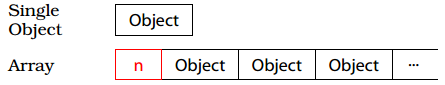
\includegraphics[width = 0.5\textwidth]{ArrayMemLayout.png}
\end{figure}

The rule is simple: if you use [] in a \texttt{new} expression, you
must use [] in the corresponding \texttt{delete} expression. If you
don't use [] in a \texttt{new} expression, don't use [] in the
matching \texttt{delete} expression.

\subsection{Store newed objects in smart pointers in standalone statements.}
\label{sec:Item-17}

Suppose we have a function to reveal our processing priority and a
second function to do some processing on a dynamically allocated
Widget in accord with a priority:

\begin{verbatim}
int priority();
void processWidget(shared_ptr<Widget> pw, int priority);
\end{verbatim}

Consider now a call to \texttt{processWidget}:
\begin{verbatim}
processWidget(new Widget, priority());
\end{verbatim}

It won't compile. \texttt{shared\_ptr'}s constructor taking a raw
pointer is \texttt{explicit}, so there's no implicit conversion. The
following code, however, will compile: 
\begin{verbatim}
processWidget(shared_ptr<Widget>(new Widget), priority());
\end{verbatim}

Although we're using object-managing resources everywhere here,
\textbf{this call may leak resources}.

Before \texttt{processWidget} can be called, then, compilers must generate
code to do these three things:
\begin{itemize}
\item Call \texttt{priority}
\item Execute \texttt{new Widget}
\item Call the \texttt{shared\_ptr} constructor
\end{itemize}

If \texttt{new Widget} expression executed before \texttt{priority()},
and  the call to \texttt{priority()} yields an exception, the pointer
returned from \texttt{new Widget} will be lost.

The way to avoid problems like this is simple: use a separate
statement to create the \texttt{Widget} and store it in a smart pointer, then
pass the smart pointer to \texttt{processWidget}:

\begin{verbatim}
shared_ptr<Widget> pw(new Widget); 
processWidget(pw, priority());
\end{verbatim}

\clearpage
\section{设计与声明}

\subsection{让接口容易被正确使用,不易被误用}
\label{sec:Item-18}

\begin{itemize}
\item 首先必须考虑客户可能做出什么错误:
\begin{verbatim}
class Date {
public:
  Date(int month, int day, int year);
  ...
};
\end{verbatim}
这就很容易以错误的次序传递参数。
\item 可以通过导入新类型来进行预防。
\begin{verbatim}
class Month {
public:
  static Month Jan() { return Month(1); } // functions returning all valid
  ... // why these are functions, not other member functions
private:
  explicit Month(int m); // prevent creation of new Month values
};
\end{verbatim}
  
\item 预防客户错误另一个办法是限制类型内什么事情可以做,什么事情不可以
  做,常见的就是加上\texttt{const},可以看Section \ref{sec:Item-3}。
\item 另一个一般性准则是尽量令types的行为与内置types一致,
\item 任何接口如果要求客户必须记得做某些事,就是有着不正确使用的可能,
  例如假如有一个\texttt{factory}函数,返回一个指针,那就有可能没有删除
  指针或者二次删除。
\begin{verbatim}
Investment* createInvestment(); 
\end{verbatim}
  我们可以返回智能指针:
\begin{verbatim}
shared_ptr<Investment> createInvestment();
\end{verbatim}
  假设class设计者要将指针传递给一个\texttt{getRidOfInvestment}来进行删
  除指针,那就要将它绑定为\texttt{shared\_ptr}的删除器:
\begin{verbatim}
shared_ptr<Investment> createInvestment(){
  shared_ptr<Investment> retVal(static_cast<Investment*>(0),
getRidOfInvestment);
  retVal = ...; // make retVal point to the correct object
  return retVal;
}
\end{verbatim}
同时,智能指针有一个特别好的性质就是消除所谓的''cross-DLL prolbem'',
这个问题发生于对象在动态链接程序库(DLL)只不过被\texttt{new}创建,却在
另一个DLL中被delete,这会导致运行期错误。 因此经常用来自动解除互斥锁
(mutex)。
\end{itemize}

\subsection{设计class犹如设计type}
\label{sec:Item-19}

\begin{itemize}
\item \textbf{新type的对象应该如何被创建和销毁?} 这会影响到构造函数、
  析构函数、内存分配函数和释放函数(\texttt{operator new, operator
    new[], operator delete, operator delete[]},见Section 8。
\item \textbf{初始化和赋值该有什么样的差别?} 不要混淆了初始化和赋值。
\item \textbf{新type的对象如果被按值传递,意味着什么?} 拷贝构造函数用
  来定义一个type的pass-by-value该如何实现。
\item \textbf{什么是新type的“合法值”?}
\item\textbf{ 新type需要配合某个继承图系(inheritance graph)吗?} 注
  意virtual和non-virtual的影响,见 Section\ref{sec:Item-34},
  Section\ref{sec:Item-36}。如果你允许其他class继承该class,那会影响你
  所声明的函数,尤其是析构函数,是否是virtual,见 Section
  \ref{sec:Item-7}。
\item \textbf{新type需要什么样的类型转换?} 如果你希望允许类型
  \texttt{T1}被隐式转换为\texttt{T2}类型,就必须在\texttt{T1}内部写一
  个类型转换函数(\texttt{operator T2}),或者在\texttt{T2}写一个
  \texttt{non-explicit-one-argument}的构造函数。
\item \textbf{什么样的操作符和函数对于新type而言是合理的?} 这决定你讲
  为你的class声明哪些函数,其中某些是member,某些不是,见 Section
  \ref{sec:Item-23},\ref{sec:Item-24},\ref{sec:Item-46}。
\item \textbf{什么样的标准函数应该驳回?} 必须声明为\texttt{private},
  见 Section \ref{sec:Item-6}。
\item \textbf{谁该取用新type的成员?} 这帮助你决定哪些成员为
  \texttt{public}、\texttt{protected}、\texttt{private},以及哪些class
  或者function应该是\texttt{friend},以及将它们嵌套于另一个之内是否合
  理。
\item \textbf{什么是新type的未声明接口(undeclared interface)?} 它对
  效率、异常安全性(Section \ref{sec:Item-29})以及资源运用(多任务锁
  定和动态内存)提供何种保证?
\item \textbf{新type有多么一般化?} 如果是定义一整个types家族,应该考
  虑模板。
\item \textbf{你真的需要一个新type吗?} 如果只是定义新的derived class
  以便为既有的class添加机能,说不定单纯定义几个non-member函数更好。
\end{itemize}

\subsection{以pass-by-reference-to-const替换pass-by-value}
\label{sec:Item-20}

\begin{itemize}
\item 以by reference-to-const方式传递参数可以减少拷贝构造和析构的开销
\item 也可以避免slicing(对象切割)的问题,即当一个derived class对象以
  by value方式传递并被视为一个base class对象。

  references在编译器底层往往以指针形式实现,因此pass-by-reference通常
  意味着真正传递的是指针。当然,如果是内置类型、STL的迭代器或者函数对
  象,pass-by-value效率更高。
\end{itemize}

\subsection{必须返回一个object时,别妄想返回其reference}
\label{sec:Item-21}

一个典型的例子就是重载算术运算符的时候不能返回reference,否则就会传递
一些references指向并不存在的对象。如果函数内部创建一个指针,就会出现内
存泄漏, 如果函数内部创建一个local static对象,那(a*b)==(c*d)永远都会
成立。

因此,\textbf{绝对不要返回pointer或者reference指向一个local stack对象或
heap-allocated对象},或者指向一个local static对象而有可能同时需要多个这
样的对象,Section \ref{sec:Item-4} 已经为“在单线程环境中合理返回
reference指向一个local static对象”提供了一份设计示例。

\subsection{将成员变量声明为private}
\label{sec:Item-22}

如果成员变量不是\texttt{public},客户唯一能够访问对象的办法就是成员函
数,这样可以保证一致性,另外,这样封装可以为“所有可能的实现”提供弹性,
例如,你可以随时修改class的实现方式,客户只需要重新编译,遵循Section
\ref{sec:Item-31}甚至可以不用重新编译。 另外,这也可以使得成员变量被读
或者被写时轻松告诉其他对象,可以验证class的约束条件以及函数的前提和时
候状态等等。

即便成员变量是\texttt{protected},如果将其取消,也会有大量不可预知的代
码受到破坏,需要重写、重新测试等等,因此,\textbf{从封装的角度,只有两
  种访问权限:private(提供封装)和其他(不提供封装)。}

\subsection{偏好non-member、non-friend来替换member函数}
\label{sec:Item-23}

\begin{verbatim}
class WebBrowser {
public:
  ...
  void clearCache();
  void clearHistory();
  void removeCookies();
  ...
  void clearEverything(); // calls clearCache, clearHistory,and removeCookies
};
void clearBrowser(WebBrowser& wb){
  wb.clearCache();
  wb.clearHistory();
  wb.removeCookies();
}
\end{verbatim}
哪一个\texttt{clearBrowser}更好呢?

面向对象守则要求数据尽可能地被封装,如果某些东西被封装,它就不再可见,
因此,越多函数可以访问数据,数据的封装性就越低。因此,当二者都可以提供
相同的机能时,选择non-member做法可以减少编译依赖度,增加class的包裹弹
性、技能扩充性。

另外一点,一个像\texttt{WebBrowser}这样的class会拥有大量便利函数,某些
与书签有关,某些与cookie有关等等,通常大多数客户指对其中某些感兴趣,一
个自然的做法是将它们分别声明于不同的头文件的相同命名空间中,这也是标准
库的组织方式,我们只需要include所需要的东西即可:
\begin{verbatim}
// header “webbrowser.h” — header for class WebBrowser itself 
// as well as “core” WebBrowser-related functionality
namespace WebBrowserStuff {
  class WebBrowser { ... };
  ... // “core” related functionality
}

// header “webbrowserbookmarks.h”
namespace WebBrowserStuff {
  ... // bookmark-related convenience functions
} 

// header “webbrowsercookies.h”
namespace WebBrowserStuff {
... // cookie-related convenience functions
}
\end{verbatim}

\subsection{如果所有参数都需要类型转换,请采用non-member函数}
\label{sec:Item-24}

考虑如果为\texttt{Rational}类重载算术运算符,如果定义为member函数,
\begin{verbatim}
Rational oneEight (1,8);
Rational result = oneEight * 2; // Correct!
Rational result = 2 * oneEight; // Error!
\end{verbatim}
因为只有被列入参数列表内的参数才可以进行隐式类型转换,所以当需要支持混
合式算术运算的时候,必须将其列为non-member函数,同时尽可能避免将其声明
为friend函数。

\textbf{如果你需要为某个函数的所有参数(包括this指针所指的隐藏参数)进
  行类型转换,这个函数就必须是non-member。}该条款并不完全成立,等牵扯
到template的时候才完整,见Section \ref{sec:Item-46}。

\subsection{考虑写一个不抛异常的swap函数}
\label{sec:Item-25}

标准库的\texttt{swap}函数十分典型:
\begin{verbatim}
namespace std {
  template<typename T> // typical implementation of std::swap;
  void swap(T& a, T& b) // swaps a’s and b’s values
  {
    T temp(a);
    a = b;
    b = temp;
  }
}
\end{verbatim}

有些时候这样做效率很低,最典型的例子就是一些“以指针指向一个对象,内涵
真正数据”的那种类型,实际上它们的\texttt{swap}只需要交换指针就可以了。

\begin{verbatim}
namespace std {
  template<> 
  void swap<Widget>(Widget& a, Widget& b){
    swap(a.pImpl, b.pImpl); // to swap Widgets, swap their pImpl pointers;
  } // this won’t compile
}
\end{verbatim}
这里试图访问Widget类的private成员,因此无法编译,正确做法是:
\begin{verbatim}
class Widget { // same as above, except for the
public: // addition of the swap mem func
  ...
  void swap(Widget& other){
     using std::swap; // the need for this declaration is explained later in this Item
     swap(pImpl, other.pImpl); // to swap Widgets, swap their
  } // pImpl pointers
  ...
};
namespace std {
  template<> // revised specialization of
  void swap<Widget>(Widget& a,Widget& b){
     a.swap(b); // to swap Widgets, call their
  } // swap member function
}
\end{verbatim}

然而当Widget和WidgetImpl都是模板类的时候还是会出现错误,因为模板函数是
不支持偏特化的,即下面的写法是不合法的:
\begin{verbatim}
namespace std {
template<typename T>
  void swap<Widget<T> >(Widget<T>& a, Widget<T>& b)
  { a.swap(b); }
}
\end{verbatim}
然而我们又不能在std namespace里面添加新东西,所以我们应该将特化的
\texttt{swap}函数和Widget类定义在一起:
\begin{verbatim}
namespace WidgetStuff {
  ... // templatized WidgetImpl, etc.
  template<typename T> // as before, including the swap
  class Widget { ... }; // member function
  ...
  template<typename T> // non-member swap function;
  void swap(Widget<T>& a,Widget<T>& b) // not part of the std namespace
  {
     a.swap(b);
  }
}
\end{verbatim}

现在,每次调用\texttt{swap}的时候都会找到该专属版本。 最后,如果你调用
\texttt{swap},请确定包含一个\texttt{using}声明式,保证
\texttt{std::swap}可见:

\begin{verbatim}
template<typename T>
void doSomething(T& obj1, T& obj2)
{
  using std::swap;
  swap(obj1, obj2); // call the best swap for objects of type T
  ...
}
\end{verbatim}

另外,成员版\texttt{swap}绝不可以抛出异常,因为\texttt{swap}的一个最好
应用就是帮助class提供强烈的异常安全性保障,Section \ref{sec:Item-29}会
提供所有细节,而它基于一个假设:成员版的\texttt{swap}绝不抛出异常。

\clearpage
\section{实现}

\subsection{尽可能延后变量定义式的出现时间}
\label{sec:Item-26}

只要定义了一个变量,就要承受构造成本和析构成本,有的时候可能会有某个变
量从未被使用,但仍会耗费成本,例如:

\begin{verbatim}
std::string encryptPassword(const std::string& password){
  using namespace std;
  string encrypted;
  if (password.length() < MinimumPasswordLength) {
    throw logic_error("Password is too short");
  }
  return encrypted;
}
\end{verbatim}

如果有个被丢出,它就真的没被使用,因此最好延后\texttt{encrypted}的定义
式:
\begin{verbatim}
std::string encryptPassword(const std::string& password){
  using namespace std;
  if (password.length() < MinimumPasswordLength) {
    throw logic_error("Password is too short");
  }
  string encrypted;
  return encrypted;
}
\end{verbatim}
但是这还不够紧实,因为\texttt{encrypted}虽然定义但没有初值,调用的是默
认构造函数,Section \ref{sec:Item-4}解释了为什么通过默认构造函数构造比
直接构造时指定初值的效率差。
\begin{verbatim}
std::string encryptPassword(const std::string& password){
  string encrypted(password); // define and initialize via copy
  encrypt(encrypted);
  return encrypted;
}
\end{verbatim}
因此“尽可能延后”是指尽可能延后到这份定义能够直接给它初值实参为止。如
果涉及循环的话,最好是放在内部,因为对程序的可理解性和易维护性更好,如
果追求效率的话就要分析赋值成本和构造析构成本哪个更高。

\subsection{少做转型动作}
\label{sec:Item-27}

转型共有五种形式:
\begin{itemize}
\item \textbf{旧式转型(old-style casts)}:
\begin{verbatim}
(T)expression //将expression转型为T
T(expression)
\end{verbatim}
\item \texttt{const\_cast<T>(expression}:通常被用来cast away the
  constness,它也是唯一由此能力的转型操作符。
\item \texttt{dynamic\_cast<T>(expression)}:主要用来执行safe
  downcasting,也是用来决定某对象是否归属集成体系中的某个类型,它是唯
  一无法用旧式语法执行的动作,也是耗费重大运行成本的动作。
\item \texttt{reinterpret\_cast<T>(expression)}:意图执行地执行低级转
  型,实际动作可能取决于编译器,例如将一个pointer to int转型为int,这
  一类在低级代码之外很少见,本书只在讨论如何针对原始内存(raw memory)写
  出一个调试用的分配器(debugging allocator)使用,见 Section
  \ref{sec:Item-50}。
\item \texttt{static\_cast<T>(expression)}:用来强迫隐式转换,例如将
  non-const对象转换为const对象,以及上述转换的反向,例如type*转换为
  void*,pointer-to-derived转为pointer-to-base等等,但是它无法将const
  转为non-const。
\end{itemize}

注意,\textbf{任何一种类型转换往往真的令编译器编译出运行期间执行的代码},
例如:
\begin{verbatim}
class Base { ... };
class Derived: public Base { ... };
Derived d;
Base *pb = &d; // implicitly convert Derived* to Base*
\end{verbatim}
这种情况下会有一个偏移量(offset)在运行期被施加于这\texttt{Derived*}
指针身上来获得正确的\texttt{Base*}指针值,这说明,单一对象可能拥有一个
以上的地址,因此你应该避免做出“object在C++中如何布局”的假设,例如,
\textbf{将object地址转型为\texttt{char*}后进行指针算术,这几乎总会导致
  无定义行为}。

关于转型还有一个有趣的事情:我们很容易写出似是而非的代码,例如
\begin{verbatim}
class Window { // base class
public:
  virtual void onResize() { ... } // base onResize impl
  ...
};
class SpecialWindow: public Window { // derived class
public:
  virtual void onResize() { // derived onResize impl;
    static_cast<Window>(*this).onResize(); // this doesn’t work!
    ...
  }
  ...
};
\end{verbatim}
此时它是在\textbf{当前对象的base class成分的副本}上调用
\texttt{Window::onResize},然后再在当前对象身上执行
\texttt{SpecialWindow}专属动作, 如果两个\texttt{onResize}修改了对
象内容,那么base class成分并没有更改,但derived class成分却更改了。解
决的办法就是:

\begin{verbatim}
class SpecialWindow: public Window {
public:
  virtual void onResize() {
    Window::onResize(); // call Window::onResize on *this
    ...
  }
  ...
};
\end{verbatim}

因此,如果你发现自己打算类别转换,这就是一个警告信号:你可能正在把局面
发展到错误的方向上,如果你用的是\texttt{dynamic\_cast}更是如此。

首先,\texttt{dynamic\_cast}执行速度相当慢,例如至少会进行多次的
\texttt{strcmp}调用来比较class名称。之所以需要\texttt{dynamic\_cast}通
常是因为你想执行derived class操作函数,但手上只有一个指向base的pointer
或者reference,有两个一般性做法可以避免这个问题:

\begin{itemize}
\item 使用容器并在其中存储直接指向derived class对象的指针(通常是智能
  指针),当然这种做法使你无法在同一个容器内存储指针指向所有可能的派生
  类,因此就需要多个容器。
\item 另一个做法就是在base class内提供virtual函数做你想对各个派生类做
  的事情。
\end{itemize}

\subsection{避免返回“handles”指向对象内部成分}
\label{sec:Item-28}

\begin{verbatim}
class Rectangle {
public:
  ...
  Point& upperLeft() const { return pData->ulhc; }
  Point& lowerRight() const { return pData->lrhc; }
  ...
};
\end{verbatim}

这两个函数被声明为const成员函数,是不想让客户修改的,但却又返回
reference指向private内部数据。这告诉我们两点:\textbf{成员变量的封装性
  最多只等于“返回其reference”的函数的访问级别}。

如果返回的是指针或者迭代器,情况是相同的,这些我们统称为
\textbf{handles},返回一个“代表对象内部数据”的handle就会带来降低封装
性的风险。因此需要将函数加上\texttt{const}。
\begin{verbatim}
class Rectangle {
public:
  ...
  const Point& upperLeft() const { return pData->ulhc; }
  const Point& lowerRight() const { return pData->lrhc; }
  ...
};
\end{verbatim}

但有时候还会存在问题,更明确地说,\textbf{它可能导致dangling handles},
比如如果返回一个指针,可能就会不小心析构了。

但这不以为绝对不可以让成员函数返回handle,有时候必须这么做,例如,
\texttt{operter[]}就是返回references指向容器内的数据。

\subsection{为异常安全而努力是值得的}
\label{sec:Item-29}

假设有个class用来表现夹带背景图案的GUI菜单,这个calss希望用于多线程,
所以有互斥器\texttt{mutex}作为并发控制用:
\begin{verbatim}
class PrettyMenu {
public:
  void changeBackground(std::istream& imgSrc); // change background image
private:
  Mutex mutex; // mutex for this object
  Image *bgImage; // current background image
  int imageChanges; // # of times image has been changed
};
\end{verbatim}
下面是\texttt{changeBackground}函数的一个可能实现:
\begin{verbatim}
void PrettyMenu::changeBackground(std::istream& imgSrc)
{
  lock(&mutex); // acquire mutex (as in Item 14)
  delete bgImage; // get rid of old background
  ++imageChanges; // update image change count
  bgImage = new Image(imgSrc); // install new background
  unlock(&mutex); // release mutex
}
\end{verbatim}
从异常安全性的观点来看,这个函数很糟糕,因为它没有满足异常安全的两个条
件:即当异常被抛出时,带有异常安全性的函数会:
\begin{itemize}
\item \textbf{不泄露任何资源。}上述代码一旦\texttt{new}出现异常,unlock就不会执行,互斥器就
  永远被hold住了。
\item \textbf{不允许数据败坏(corrupted)。}如果\texttt{new}出现异常,
  \texttt{bgImage}就会指向一个已被删除的对象,\texttt{imageChanges}也
  被累加,但新图像并没有成功安装。
\end{itemize}

解决资源泄露很容易,可以看Section \ref{sec:Item-13},\ref{sec:Item-14}。

在专注解决数据败坏之前,先定义一些术语:
异常安全函数(Exception-safe functions)提供以下三个保证之一:
\begin{itemize}
\item \textbf{基本承诺:}如果异常被抛出,程序内任何事物仍然保持在有效
  状态,所有对象都处于内部前后一致的状态。举个例子,如果有异常抛出,
  \texttt{PrettyMenu}对象可以继续拥有原背景图像或者拥有一个默认图像。
\item \textbf{强烈保证:}如果异常被抛出,程序状态不改变,即如果函数失
  败,程序会回复到“调用函数之前”的状态。和这样的函数共事是最容易的。
\item \textbf{不抛掷(nothrow)保证:}承诺不抛出异常,因为它们总是能够
  完成承诺的功能。作用于内置类型(int,指针等等)的所有操作都提供
  nothrow保证。
\begin{verbatim}
int doSomething() noexcept;
int doSomething() throw();
\end{verbatim}
这并不是说\texttt{doSomething}绝对不会抛出异常,而是说抛出异常是严重的
错误。
\end{itemize}

因此,我们目前的抉择是,我们该为我们所写的函数提供哪一种保证?从异常安
全性的观点看来,\texttt{nothrow}函数很棒,但是大部分函数而言,抉择往往
在基本保证和强烈保证之间。

对于\texttt{changebackground}而言,提供强烈保证不困难:不仅将
\texttt{Image*}改为智能指针,还重新排列了一下语句次序,在更换图像之后
才累加\texttt{imageChanges}。
\begin{verbatim}
class PrettyMenu {
  ...
  std::tr1::shared_ptr<Image> bgImage;
  ...
};
void PrettyMenu::changeBackground(std::istream& imgSrc){
  Lock ml(&mutex);
  bgImage.reset(new Image(imgSrc));
  ++imageChanges;
}
\end{verbatim}

另外,还有一个一般化的设计策略可以做到强烈保证:\textbf{copy and swap}
: 
为你打算修改的object做出一个副本,然后在副本上修改,如果有任何动作抛出
异常,原object则保持不变。待所有改变成功后,再将副本与原object进行swap
。 实现上通常是将所有“隶属对象的数据”从原object放进另一个对象内,然
后赋予原object一个指针指向哪个所谓的实现对象(implementation object,
即副本),这种手法通常被叫做\textbf{pimpl idiom},可见Section
\ref{sec:Item-31}。对\texttt{PrettyMenu}而言,写法如下:
\begin{verbatim}
struct PMImpl { 
  std::tr1::shared_ptr<Image> bgImage;
  int imageChanges; 
};
class PrettyMenu {
private:
  Mutex mutex;
  std::tr1::shared_ptr<PMImpl> pImpl;
};
void PrettyMenu::changeBackground(std::istream& imgSrc){
  using std::swap; // see Item 25
  Lock ml(&mutex); // acquire the mutex
  std::tr1::shared_ptr<PMImpl> pNew(new PMImpl(*pImpl));
  pNew->bgImage.reset(new Image(imgSrc)); // modify the copy
  ++pNew->imageChanges;
  swap(pImpl, pNew); // swap the new data into place
} // release the mutex
\end{verbatim}

但是并非所有函数都能够这样来实现“强烈保证”。另外,它并不能保证整个函
数是有强烈的异常安全性的:
\begin{verbatim}
void someFunc()
{
  f1();
  f2();
}
\end{verbatim}
只要其中一个无法提供异常安全保证,整体就无法提供异常安全保证。
\textbf{函数提供的“异常安全保证”通常最高值等于各个函数的“异常安全保
  证”中的最弱者。}

\subsection{透彻理解inline的里里外外}
\label{sec:Item-30}

\texttt{inline}的好处有:
\begin{itemize}
\item 减少了函数调用所导致的额外开销。
\item 编译器最优化机制被设计用来浓缩那些“不含函数调用”的代码,因此编
  译器用能力对inline函数本体执行语境相关最优化。
\item 如果对各种函数都用\texttt{inline}的话,目标代码(object code)会
  增加,可能会导致额外的换页行为(paging),降低指令高速缓存装置的击中
  率(instruction cache hit rate)以及伴随而来的效率。 反过来讲,如果
  inline函数本体很小,那么编译器产出的object code可能会更小,就会更好
  的效率。
\end{itemize}

\texttt{inline}只是对编译器的申请,也可以隐式提出,隐式方式就是将函数
定义在class定义中,friend函数同样适用。
\begin{verbatim}
class Person {
public:
  ...
  int age() const { return theAge; }
private:
  int theAge;
};

template<typename T> // an explicit inline
inline const T& std::max(const T& a, const T& b)
{ return a < b ? b : a; } 
\end{verbatim}

template和inline函数都要放在头文件中,因为编译器要将其具现化或者替换函
数调用的时候必须知道函数长什么样子。同时,\textbf{编译器拒绝将太复杂的
  函数inlining(例如带有循环和递归),对于所有virtual函数的调用也都会
  拒绝inlining。} 幸运的是:如果编译器无法inline,会给你一个警告信息
(见Section \ref{sec:Item-53})。

还有些时候编译器虽有意愿inline某个函数,但也还可能会为该函数生成一个函
数本体:
\begin{itemize}
\item 如果程序要取某个inline函数的地址,编译器就必须为此函数生成一个函
  数本体,编译器通常不对通过函数指针调用的inline函数实施inlining。即
  inline函数的调用有可能被inlined,也可能不被inlined。
\item 有时候编译器会生成构造函数和析构函数的outline副本,这样它们就可
  以获得函数指针用在array内部元素的构造和析构过程中。
\end{itemize}

然而,声明inline也是有成本的:
\begin{itemize}
\item 首先是代码膨胀。
\item 其次,\textbf{析构函数和构造函数往往是inline的糟糕候选
  人},虽然表面上构造函数是空的或者很少,实际上所有对象都要初始化以及
异常处理都是构造函数要提供的行为,如果是继承类的构造函数inline,那么基
类的构造函数代码也会被插入进来。
\item 另外,inline函数无法随着程序库的升级而升级:假设f是一个inline函
  数,如果f改变了,所有涉及到f的程序都需要重新编译。如果f不是inline函
  数,程序只需要重新链接就好。
\item 最后,大部分调试器对inline函数都束手无策,因为无法对并不存在的函
  数设立断点。
\end{itemize}

\subsection{将文件间的编译依存关系降到最低}
\label{sec:Item-31}
\begin{verbatim}
class Person {
public:
  Person(const std::string& name, const Date& birthday, const Address& addr);
  std::string name() const;
  std::string birthDate() const;
  std::string address() const;
  ...
private:
  std::string theName; // implementation detail
  Date theBirthDate; // implementation detail
  Address theAddress; // implementation detail
};
\end{verbatim}
一旦某个类型发生改变,所有含\texttt{Person}的文件都要重新编译。 我们可
以采用\textbf{pimpl idiom (pointer to implementation)}的设计:
\begin{verbatim}
class PersonImpl; // forward decl of Person impl. class
class Date; // forward decls of classes used in
class Address; // Person interface
class Person {
public:
  Person(const std::string& name, const Date& birthday, const Address& addr);
  std::string name() const;
  std::string birthDate() const;
  std::string address() const;
  ...
private:
  shared_ptr<PersonImpl> pImpl;
};
\end{verbatim}
在这样的设计下,\texttt{Person}的客户就完全与其他类的实现细节相分离了。
这个分离的关键在于以“声明的依存性”替换“定义的依存性”,那正是编译依
存性最小化的本质:\textbf{让头文件尽可能自我满足,万一做不到,则让它与
  其他文件内的声明式(而非定义式)相依}。其他每一件事都源自于这个简单
的设计策略:
\begin{itemize}
\item 如果使用object reference或者pointer就可以完成任务,就不要使用
  object。
\item 尽量以class声明式替换class定义式:当你声明一个函数而它要用到某个
  class时,并不需要该class的定义,加一个前置class声明就可以。
\begin{verbatim}
class Date;
Date today();
void clearAppointments(Date d); //不需要Date的定义式
\end{verbatim}
\item 为声明式和定义式提供不同的头文件。
\end{itemize}

像上面的pimpl idiom的classes经常被称为\textbf{Handle classes},另一个
制作Handle class的方法是令\texttt{Person}成为一种特殊的抽象基类,称为
\textbf{Interface class}。
\begin{verbatim}
class Person {
public:
  virtual ~Person();
  virtual std::string name() const = 0;
  virtual std::string birthDate() const = 0;
  virtual std::string address() const = 0;
  static shared_ptr<Person> create(const std::string& name, const Date& birthday, const Address& addr); 
  ...
};

class RealPerson: public Person {
public:
  RealPerson(const std::string& name, const Date& birthday, const Address& addr)
  : theName(name), theBirthDate(birthday), theAddress(addr){}
  virtual ~RealPerson() {}
  std::string name() const; // implementations of these
  std::string birthDate() const; // functions are not shown, but
  std::string address() const; // they are easy to imagine
private:
  std::string theName;
  Date theBirthDate;
  Address theAddress;
};

shared_ptr<Person> Person::create(const std::string& name, const Date&birthday, const Address& addr)
{
  return shared_ptr<Person>(new RealPerson(name, birthday,addr));
}
\end{verbatim}

当然,它们也都是有成本代价的,handle classes会增加内存大小,会为每一次
访问增加一层间接性,也要承受初始化,释放的额外开销和异常可能。

Interface classes每个函数都是\texttt{virtual},所以每次函数调用都要付
出一个间接跳跃(indirect jump)成本(见Section \ref{sec:Item-7}),另
外也要承担vptr带来的额外内存。

最后,\textbf{Handle classes和Interface classes脱离inline函数就没有什
  么作为},因为只有inline函数本体才必须要置于头文件内部,它们正是特别
被设计用来隐藏实现细节的。当它们导致速度或大小差异过于重大以至于class
之间的耦合并不成为关键时,我们就用具象类(concrete class)替换handle
class和interface class。

\clearpage
\section{继承与面向对象设计}

\subsection{确定你的public继承塑模出is-a关系}
\label{sec:Item-32}

\texttt{public}继承意味着is-a关系,适用于base classes身上的每一件事情
一定也适用于derived class身上。例如:企鹅是不会飞的鸟,但大部分鸟会飞。
这样三层继承关系比较合适:
\begin{verbatim}
class Bird {
  ... // no fly function is declared
};
class FlyingBird: public Bird {
public:
  virtual void fly();
  ...
};
class Penguin: public Bird {
  ... // no fly function is declared
};
\end{verbatim}

当然,也有一种处理方式是为企鹅定义fly函数,令它产生一个运行期错误:
\begin{verbatim}
class Penguin: public Bird {
public:
  virtual void fly() { error("Attempt to make a penguin fly!"); }
  ...
};
\end{verbatim}

Section \ref{sec:Item-18}说过:\textbf{好的接口可以防止无效的代码通过
  编译},所以第一种是更好的选择。

\subsection{避免遮掩(hide)继承而来的姓名}
\label{sec:Item-33}

关于name hiding看Section \ref{sec:Overload}。

有时候你并不想继承base class的所有函数,在public继承下是绝对不可能的,
但是在private继承下是可以的:
\begin{verbatim}
class Base {
public:
  virtual void mf1();
  virtual void mf1(int);
  ... // as before
};
class Derived: private Base {
public:
  virtual void mf1(){ Base::mf1(); } 
};
...
Derived d;
int x;
d.mf1(); // fine, calls Derived::mf1
d.mf1(x); // error! Base::mf1() is hidden
\end{verbatim}
这里无法用using,因为它会令所有基类同名函数在继承类中都可见。我们将其
称之为\textbf{inline转交函数(forwarding function)}。

假如继承结合template,就将面对“继承名称被遮掩”的一个全然不同的形式,
到时候再讲,可见Section \ref{sec:Item-43}。

\subsection{区分接口继承和实现继承}
\label{sec:Item-34}

看下面这个例子:
\begin{verbatim}
class Shape {
public:
  virtual void draw() const = 0;
  virtual void error(const std::string& msg);
  int objectID() const;
  ...
};
class Rectangle: public Shape { ... };
class Ellipse: public Shape { ... };
\end{verbatim}

将函数定义为pure virtual函数,impure virtual函数,non-virtual函数分别
对应着你想要derived class继承的东西:
\begin{itemize}
\item 只继承接口,每一个shape继承类都有其独自的draw实现。
\item 继承接口和一份缺省实现,每一个继承类可以重写,但如果不重写,也可
  以使用基类的实现。
\item 继承接口和一份强制实现,每一个继承类都不应该修改该实现。
\end{itemize}

这里有一个小tip注意一下:pure virtual函数也是可以定义的,继承类可以用
\texttt{Base::virtualFunction()}来调用。

这样可以避免经验不足的class设计者常犯的两个错误:
\begin{itemize}
\item 将所有函数声明为non-virtual,这使得继承类无法进行特化,析构函数
  也会带来问题。
\item 将所有成员函数都声明为virtual,有时候这样是对的,例如interface
  class,但是这也可能是设计者缺乏坚定立场的前兆。某些函数就是不该在继
  承类中重新被定义,就应该将它声明为non-virtual。
\end{itemize}


\subsection{考虑virtual函数以外的其他选择}
\label{sec:Item-35}

\begin{verbatim}
class GameCharacter {
public:
  virtual int healthValue() const;
};
\end{verbatim}

还有两种设计可以替代这种virtual函数:
\begin{itemize}
\item \textbf{借助non-virtual interface(NVI)}来实现\textbf{template method}
  模式:
\begin{verbatim}
class GameCharacter {
public:
  int healthValue() const{ // derived classes do not redefine
    ... // do “before” stuff — see below
    int retVal = doHealthValue(); // do the real work
    ... // do “after” stuff — see below
    return retVal;
}
private:
  virtual int doHealthValue() const{ // derived classes may redefine this
    ... // default algorithm for calculating character’s health
  }
};
\end{verbatim}
  我们把这个non-virtual函数称为virtual函数的外包装(wrapper)。这种设
  计的优缺点在于:
  \begin{itemize}
  \item 可以在wrapper之前和之后做一些事情,例如验证函数的先决条件和事
    后条件等等,如果让客户直接调用virtual函数就没有办法做到这个事情。
  \item 但是NVI设计涉及在继承类内重新定义若干个继承类并不会调用的
    virtual函数。
  \item 在NVI手法下并不一定需要virtual函数是private的,假如继承类也需
    要调用基类函数,就必须是protected。有时候virtual函数甚至一定得是
    public,例如析构函数,这样就不能实施NVI手法了。
  \end{itemize}
  
\item 第二个是\textbf{藉由Function Pointers实现Strategy模式}。
\begin{verbatim}
class GameCharacter; // forward declaration
// function for the default health calculation algorithm
int defaultHealthCalc(const GameCharacter& gc);
class GameCharacter {
public:
  typedef int (*HealthCalcFunc)(const GameCharacter&);
  explicit GameCharacter(HealthCalcFunc hcf = defaultHealthCalc): healthFunc(hcf){}
  int healthValue() const
  { return healthFunc(*this); }
  ...
private:
  HealthCalcFunc healthFunc;
};
\end{verbatim}
  这种设计模式提供了某些有趣弹性:
  \begin{itemize}
  \item 同一类型的不同实体可以有不同的健康计算函数。
  \item 某一直任务的健康计算函数可以在运行期变更,即这些计算函数并未访
    问对象的non-public成分。如果计算需要用到non-public成分,就需要弱化
    class的封装,例如声明friend或者提供一些public访问函数等。 
  \end{itemize}

\item 还可以藉由\texttt{function}完成\textbf{strategy模式}:
\begin{verbatim}
class GameCharacter; // as before
int defaultHealthCalc(const GameCharacter& gc); // as before
class GameCharacter {
public:
  typedef std::function<int (const GameCharacter&)> HealthCalcFunc;
  explicit GameCharacter(HealthCalcFunc hcf = defaultHealthCalc):healthFunc(hcf){}
  int healthValue() const
  { return healthFunc(*this); }
  ...
private:
  HealthCalcFunc healthFunc;
};
\end{verbatim}
  \texttt{std::function}使得“健康计算函数”具有更大的弹性:
\begin{verbatim}
short calcHealth(const GameCharacter&); //non-int return type
struct HealthCalculator { // class for health
  int operator()(const GameCharacter&) const // calculation function objects
  { ... }
};
class GameLevel {
public:
  float health(const GameCharacter&) const;
}; 
class EvilBadGuy: public GameCharacter { // as before
  ...
};
GameLevel currentLevel;
EvilBadGuy ebg(std::bind(&GameLevel::health,currentLevel,_1));
\end{verbatim}
  \texttt{GameLevel::health}实际上有两个参数,有一个隐式参数
  \texttt{*this},如果我们将它作为a将抗击孙函数,就必须用某种方式转换
  它,使它不再接受两个参数,于是我们将\texttt{currentLevel}作为第一个
  参数输入,这个就是\texttt{std::bind}做的事情。
\item 最后一点就是可以将集成体系内的virtual函数替换为另一个集成体系内
  的virtual函数,比如,关于健康计算可以创建一个继承体系,人物部分再用
  \texttt{std::function}实现strategy模式即可。
\end{itemize}

\subsection{绝不重新定义继承而来的non-virtual函数}
\label{sec:Item-36}
\begin{verbatim}
class B {
public:
  void mf();
};
class D: public B {
public:
  void mf(); // hides B::mf; see Item 33
};

D x;
B *pB = &x;
D *pD = &x;
pB->mf(); // calls B::mf
pD->mf(); // calls D::mf
\end{verbatim}

\subsection{绝不重新定义继承而来的缺省参数值}
\label{sec:Item-37}

\textbf{virtual函数是动态绑定,但是缺省参数值却是静态绑定}:
\begin{verbatim}
class Shape {
public:
  enum ShapeColor { Red, Green, Blue };
  virtual void draw(ShapeColor color = Red) const = 0;
};
class Rectangle: public Shape {
public:
// notice the different default parameter value — bad!
virtual void draw(ShapeColor color = Green) const;
...
};
class Circle: public Shape {
public:
virtual void draw(ShapeColor color) const;
...
};

Circle *pc = new Circle; 
Shape *pr = new Rectangle;
pc->draw(); // Error! No default parameter!
pr->draw(); // calls Rectangle::draw(Shape::Red)!
\end{verbatim}
\textbf{虽然pr执行的是Rectangle的draw,但是缺省参数值却是来自Shape
  class的。}这是编译器为了保证运行期效率所采用的行为。

但是我们真的要每一个继承类都要重新写一下相同的缺省参数值,类似下面这种
的吗?
\begin{verbatim}
class Rectangle: public Shape {
public:
  virtual void draw(ShapeColor color = Red) const;
};
\end{verbatim}
这样会代码重复,并且又有相依性,一旦基类缺省值作了修改,所有继承类都要
修改。一种替代设计就是Section \ref{sec:Item-35}讲到的NVI手法:令base
class内的一个public non-virtual函数调用private virtual函数,后者可被
derived class重新定义。
\begin{verbatim}
class Shape {
public:
  enum ShapeColor { Red, Green, Blue };
  void draw(ShapeColor color = Red) const{
    doDraw(color); // calls a virtual
  }
private:
  virtual void doDraw(ShapeColor color) const = 0; 
};
class Rectangle: public Shape {
public:
  ...
private:
  virtual void doDraw(ShapeColor color) const;
};
\end{verbatim}

\subsection{通过composition塑模出has-a关系或者“根据某物实现出”关系}
\label{sec:Item-38}

composition指的是某种类型的对象内含有其他类型的对象,同义词还有
layering, containment, aggregation, embedding。

程序中的对象相当于你塑造的某种事物,这属于应用域(application domain)
部分,还有一些对象则是纯粹实现细节上的人工制品,例如缓冲区buffers,互
斥器mutexes,查找树search trees等等,这些相当于实现域(implementation
domain),当复合发生在这两个区域内,就表现出has-a或者
is-implemented-in-terms-of关系。
\textbf{has-a和is-a很好区分,但是is-a和is-implemented-in-terms-of比较
  麻烦。}
例如,当你想利用list实现一个set,这就不能用继承关系,而是要用复合。


\subsection{明智而审慎使用private继承}
\label{sec:Item-39}

private继承实际上意味着implemented-in-terms-of。D以private形式继承B,
意味着D对象是根据B对象实现而得,并没有其他意义了。

Section~\ref{sec:Item-38}提到compo sition也有同样的意义,那么怎么做取舍
呢?答案很简单:\textbf{尽可能使用复合,必要时才使用private继承,主要
  是当protected成员或者virtual函数牵扯进来的时候,还有一种激进情况是空
  间方面的利害关系。}

假设我们的程序涉及\texttt{Widgets},我们需要涉及某种定时器来收集它的数
据,此时我们有工具:
\begin{verbatim}
class Timer {
public:
  explicit Timer(int tickFrequency);
  virtual void onTick() const; // automatically called for each tick
};
\end{verbatim}

此时我们有两种设计:
\begin{itemize}
\item \textbf{private继承:}
\begin{verbatim}
class Widget: private Timer {
private:
  virtual void onTick() const; // look at Widget usage data, etc.
};
\end{verbatim}
\item \textbf{public继承+复合:}
\begin{verbatim}
class Widget {
private:
  class WidgetTimer: public Timer {
  public:
    virtual void onTick() const;
  };
  WidgetTimer timer;
  ...
};
\end{verbatim}
\end{itemize}

第二种设计是更好的,原因在于:
\begin{itemize}
\item 首先,你之后可能会想设计\texttt{Widget}使它得以拥有继承类,同时
  你可能会想阻止继承类重新定义\texttt{onTick},这种想法只有第二种设计
  可以做到。
\item 你可能会想将Widget的编译依存性降低,那么我们就可以把WidgetTimer
  移出Widget之外,Widget内含一个WidgetTimer指针即可,这样Widget就不再
  需要include任何与Timer有关的东西。
\end{itemize}

之前提到的激进情况针对于空白类,即内部没有任何数据,包括non-static成员,
virtual函数,也没有virtual base class:
\begin{verbatim}
class Empty {};
class HoldAnInt {
private:
  int x;
  Empty e;
};
sizeof(HoldsAnInt) > sizeof(int) !!!
\end{verbatim}
你会发现很神奇的事情是,\texttt{HoldsAnInt}的size会大于一个int,因为
\texttt{size(Empty)=1},有时候编译器为了齐位,\texttt{size(Empty)}可能
等于\texttt{size(int)}。

但是如果我们继承Empty:
\begin{verbatim}
class HoldsAnInt: private Empty {
private:
  int x;
};
\end{verbatim}
可以发现\texttt{sizeof(HoldsAnInt)==sizeof(int)},这就是空白基类最优化
(EBO,empty base optimization)。

现实中的empty class并不一定是empty,它们可能包含typedefs,enums,
static成员变量或者non-virtual函数。STL中就有许多技术用途的empty class,
EBO使得这样的继承很少增加继承类的大小。

\subsection{明智而审慎使用多重继承}
\label{sec:Item-40}

最先要认清的一件事是程序有可能会从多个base class里继承相同名称,从而导
致歧义(ambiguity):
\begin{verbatim}
class BorrowableItem { 
public:
  void checkOut(); // check the item out from the library
};
class ElectronicGadget {
private:
  bool checkOut() const;
};
class MP3Player: public BorrowableItem, public ElectronicGadget{ ... }; 
MP3Player mp;
mp.checkOut(); // ambiguous!
mp.BorrowableItem::checkOut();
\end{verbatim}

多重继承中最要命的是钻石型多重继承:
\begin{verbatim}
class File { ... };
class InputFile: public File { ... };
class OutputFile: public File { ... };
class IOFile: public InputFile, public OutputFile{ ... };
\end{verbatim}
这时候有一个问题:base class内的成员变量是否要经由每一条路径复制?从一
个角度说,对于File中的变量fileName,IOFile应该有两份fileName成员变量,
但另一个角度说,IOFile对象只该有一个文件名称。\textbf{C++默认第一种,
  如果想要第二种,只需要让InputFile和OutputFile进行virtual继承即可。}

从正确行为观点看,public继承应该总是virtual的,但是virtual继承需要付出
很多代价:
\begin{itemize}
\item virtual继承的那些class所产生的对象往往比non-virtual的大。
\item 初始化规则复杂且不直观:virtual base初始化责任是由most derived
  class负责的。
\end{itemize}
但是还是非必要不使用virtual base,如果使用就尽可能避免在base class中防
放置数据。

\clearpage
\section{模板与泛型编程}

\subsection{了解隐式接口和编译期多态}
\label{sec:Item-41}

前面讲的都是显式接口(explicit interface)和运行期多态(runtime
polymorphism),即virtual函数。 但是template而言是隐式接口和编译期多态
。这类似于“哪一个重载函数该被调用(编译期发生)”和“哪一个virtual函
数该被绑定(运行期发生)”的差异。

\subsection{了解typename的双重意义}
\label{sec:Item-42}

在template声明式中class和typename没有不同。但有一些情况必须要用
typename。

\begin{verbatim}
template<typename C> // print 2nd element in
void print2nd(const C& container){ // this is not valid C++!
  if (container.size() >= 2) {
    C::const_iterator iter(container.begin());
    ++iter;
    int value = *iter;
    std::cout << value;
  }
}
\end{verbatim}

template内出现依赖于某个template参数,称之为\textbf{从属名
  称}(dependent names),反之为\textbf{非从属名称(non-dependent
  names)}。如果从属名称在class内呈嵌套状,则称作
\textbf{嵌套(nest)从属名称},\texttt{C::const\_iterator}就是这种名称。

嵌套从属名称可能会导致解析(parsing)困难:如果C有个static成员变量而碰
巧命名为\texttt{const\_iterator}呢?那么,想要告诉编译器这是一个类型的
话,就必须在他之前加上关键字\texttt{typename}。

一般性规则很简单:任何时候你想在template中指涉一个嵌套从属类型名称,就
必须加上关键字\texttt{typename},例如:
\begin{verbatim}
template<typename C> // typename allowed (as is “class”)
void f(const C& container, // typename not allowed
typename C::iterator iter); // typename require
\end{verbatim}

但该规则的一个例外是:\texttt{typename}不可以出现在base class list内的
嵌套从属类型名称之前,也不可以在member initialization list中作为base
class的修饰符,例如:
\begin{verbatim}
template<typename T>
class Derived: public Base<T>::Nested { // base class list: typename not allowed
public: 
  explicit Derived(int x) : Base<T>::Nested(x) // base classidentifier in mem. init. list: typename not allowed
  {
    typename Base<T>::Nested temp; // use of nested dependent type
  }
};
\end{verbatim}

最后再看一个\texttt{typename}的例子:
\begin{verbatim}
template<typename IterT>
void workWithIterator(IterT iter){
  typename std::iterator_traits<IterT>::value_type temp(*iter);
  ...
}
\end{verbatim}

\subsection{学习处理模板化基类内的名称}
\label{sec:Item-43}

\begin{verbatim}
class CompanyA {
public:
  ...
  void sendCleartext(const std::string& msg);
  void sendEncrypted(const std::string& msg);
  ...
};

template<typename Company>
class MsgSender {
public:
  ... // ctors, dtor, etc.
  void sendClear(const MsgInfo& info){
    std::string msg;
    create msg from info;
    Company c;
    c.sendCleartext(msg);
  }
  void sendSecret(const MsgInfo& info){ ... }
};
\end{verbatim}

如果我们想每次发信息的时候要记录某些东西,我们会想出这样的解法:
\begin{verbatim}
template<typename Company>
class LoggingMsgSender: public MsgSender<Company> {
public:
  void sendClearMsg(const MsgInfo& info){
    write "before sending" info to the log;
    sendClear(info); // call base class function;
    // this code will not compile!
     write "after sending" info to the log;
  }
  ...
};
\end{verbatim}

这里我们换了一个不同的名称,这样既可以避免遮掩继承而得的名称,也避免重
新定义一个继承而得的non-virtual函数。但是,以上代码无法通过编译,问题
在于,编译器在遇到class template LoggingMsgSender定义式时,并不知道它
继承什么样的class,更明确地说,编译器没办法知道它是否有
\texttt{sendClear}函数。因此,\textbf{编译器往往拒绝在templatized base
  class内寻找继承而来的名称。}

\textbf{编译器编译期会去解析与模板无关的名称(都是静态绑定),运行期再
  去解析与模板相关的名称,但不会进入templatized base class内寻找名称。} 

\begin{verbatim}
void g() { cout<<"gobal::g()"<<endl; }

template<class T> class X {
public:
  void g() { cout<<"X::g()"<<endl; }
};

//Use of undeclared identifer g if global g() has been commented out.
template<class T> class Y : public X<T> {
public:
  void f() { g(); this->g(); }
};

template<> class Y<char> : public X<char> {
public:
  void f() { g(); this->g(); }
};

Y<char> y;
y.f(); \\ X::g() X::g()
Y<int> y;
y.f(); \\ global::g() X::g()
\end{verbatim}

我们有三种方法可以让C++“不进入templatized base classes观察”的行为失
效:
\begin{itemize}
\item 在base class函数调用动作之前加上\texttt{this->}:
\begin{verbatim}
void sendClearMsg(const MsgInfo& info){
  write "before sending" info to the log;
  this->sendClear(info); // okay, assumes that
  // sendClear will be inherited
  write "after sending" info to the log;
}
\end{verbatim}
\item 使用\texttt{using}声明式:
\begin{verbatim}
using MsgSender<Company>::sendClear; // tell compilers to assume that sendClear is in the base class
void sendClearMsg(const MsgInfo& info){
  ...
  sendClear(info); // okay, assumes that sendClear will be inherited
  ... // 
}
\end{verbatim}
\item 指出被调用的函数位于base class内部:
\begin{verbatim}
void sendClearMsg(const MsgInfo& info){
  ...
  MsgSender<Company>::sendClear(info);
  ... 
}
\end{verbatim}
  但这样会关闭virtual绑定行为。
\end{itemize}

上述每一个解法都在\textbf{对编译器承诺,base class template的任何特化
  版本都将支持其一般版本所提供的借口。}

\subsection{将与参数无关的代码抽离templates}
\label{sec:Item-44}

\begin{verbatim}
template<typename T, std::size_t n> 
class SquareMatrix {
public:
  ...
  void invert(); // invert the matrix in place
};
\end{verbatim}

当n不同时会产生多个invert()函数,这个是重复的,因此我们可以这样解决:
\begin{verbatim}
template<typename T>
class SquareMatrixBase {
protected:
  SquareMatrixBase(std::size_t n, T *pMem) : size(n), pData(pMem) {} 
  void setDataPtr(T *ptr) { pData = ptr; } // reassign pData
  ...
private:
  std::size_t size; // size of matrix
  T *pData; // pointer to matrix values
};

template<typename T, std::size_t n>
class SquareMatrix: private SquareMatrixBase<T> {
public:
  SquareMatrix() : SquareMatrixBase<T>(n, 0), /pData(new T[n*n])
  { this->setDataPtr(pData.get()); } //give a copy of it to the base class
private:
  boost::scoped_array<T> pData; // see Item 13 for info on
};
\end{verbatim}

\subsection{运用成员函数模板接受所有兼容类型}
\label{sec:Item-45}

真实指针做得很好的一件事是支持隐式转换:Derived class指针可以隐式转换
为base class指针,non-const对象指针可以转换为const对象的指针等等。但是
智能指针比较麻烦,因为同一个template的不同instantiations之间没有固有关
系。

我们可以使用member function templates:
\begin{verbatim}
template<typename T>
class SmartPtr {
public:
  template<typename U>
  SmartPtr(const SmartPtr<U>& other)
  : heldPtr(other.get()) { ... } 
  T* get() const { return heldPtr; }
  ...
private:
  T *heldPtr;
};
\end{verbatim}
这个行为只有当坐在某个隐式转换的时候才能通过编译,这正是我们想要的。

除了构造函数,这种方法也支持赋值操作。但有一点要注意:如果你声明
member template用于拷贝构造或赋值操作,你还是要声明正常的拷贝构造函数
和拷贝赋值操作符。
\begin{verbatim}
template<class T> class shared_ptr {
public:
  template<class Y> 
  explicit shared_ptr(Y * p);
  template<class Y> 
  shared_ptr(shared_ptr<Y> const& r); 
  template<class Y> 
  explicit shared_ptr(weak_ptr<Y> const& r);
  template<class Y>
  explicit shared_ptr(auto_ptr<Y>& r); //there is not const!
  template<class Y>
  shared_ptr& operator=(shared_ptr<Y> const& r);
  template<class Y> 
  shared_ptr& operator=(auto_ptr<Y>& r); 
\end{verbatim}
从某个内置指针或者智能指针类型另一个\texttt{shared\_ptr}类型是不允许的。
\texttt{auto\_ptr}是并未被声明为const的。

\subsection{需要类型转换时将模板定义为非成员函数}
\label{sec:Item-46}

Section \ref{sec:Item-46}讨论过为什么只有non-member函数才有能力在所有
实参上实施隐式类型转换,在这里我们将其模板化了。

\begin{verbatim}
template<typename T>
class Rational {
public:
  Rational(const T& numerator = 0, const T& denominator = 1); 
  const T numerator() const; 
  const T denominator() const;
};
template<typename T>
const Rational<T> operator*(const Rational<T>& lhs, const Rational<T>& rhs)
{ ... }

Rational<int> oneHalf(1, 2); 
Rational<int> result = oneHalf * 2; // error! won’t compile
\end{verbatim}

在调用operator*的时候,编译器并不知道我们想要调用什么函数,它需要想出
什么函数被operator*的template具现化出来,所以需要先算出T是什么,但是
\textbf{template的实参推导规程并不考虑“通过构造函数而发生的”隐式类型
  转换。}

解决办法就是在template class内使用friend声明式:

\begin{verbatim}
template<typename T>
class Rational {
public:
  ...
  friend const Rational operator*(const Rational& lhs, const Rational& rhs); 
};
template<typename T> 
const Rational<T> operator*(const Rational<T>& lhs, const Rational<T>& rhs)
{ ... }
\end{verbatim}

当\texttt{oneHalf}被声明为一个\texttt{Rational<int>}的时候,
\texttt{class Rational<int>}也被具现化出来,同时friend函数也就被自动声
明出来,它此时只是一个函数而非函数模板,因此编译器调用他的时候就可以使
用隐式转换函数了。

但此时能通过链接,但是无法编译,因为这个函数只被声明于类内部,并没有被
定义出来,\textbf{最简单的可行办法就是将\texttt{operator*}本体合并至声
  明式内部。}

这个技术的一个趣味点是:我们虽然用friend,却与其传统用途“访问class的
non-public”成分毫不相干。为了让类型转换发生于所有实参上,我们需要
non-member函数;为了令函数被自动具现化,需要声明在class内部,而在class
内部声明一个non-member函数的唯一办法就是friend。

正如Section~\ref{sec:Item-30}所说,定义在class内部的函数都会成为inline,
为了减少这种inline声明带来的冲击,我们可以让\texttt{operator*}不作任何
事情,让它去调用辅助函数:
\begin{verbatim}
template<typename T> class Rational;
template<typename T> 
const Rational<T> doMultiply( const Rational<T>& lhs, const
Rational<T>& rhs);
template<typename T>
class Rational {
public:
  ...
  friend const Rational<T> operator*(const Rational<T>& lhs,
const Rational<T>& rhs)
  { return doMultiply(lhs, rhs);
  ...
};
\end{verbatim}

\subsection{使用traits classes表现类型信息}
\label{sec:Item-47}

STL有五种迭代器:
\begin{itemize}
\item \textbf{Input迭代器}只能向前移动,一次一步,客户只能读取它们所指
  的东西,且只能读取一次,例如\texttt{istream\_iterators}
\item \textbf{Output迭代器}类似,例如\texttt{ostream\_iterators},他们
  俩只适合一次性操作算法(one-pass algorithms)
\item \textbf{forward}迭代器可以做前面的事情,也可以读或写一次以上,使
  得它们可以用于多次性操作算法,例如单向linked list的迭代器,
\item \textbf{Bidirectional迭代器}可以双向移动,例如STL的
  list, set, multiset, map, multimap的迭代器。
\item \textbf{random access迭代器},它最有威力,因为它可以执行迭代器算
  术:在常量时间内向前或向后跳跃人以距离,例如vector, dequem string的
  迭代器。
\end{itemize}
对于这五种分类,STL分别提供专属的卷标结构(tag struct)加以确认:
\begin{verbatim}
struct input_iterator_tag {};
struct output_iterator_tag {};
struct forward_iterator_tag: public input_iterator_tag {};
struct bidirectional_iterator_tag: public forward_iterator_tag {};
struct random_access_iterator_tag: public bidirectional_iterator_tag {};
\end{verbatim}

如果我们想实现advance函数来将迭代器移动某个距离:
\begin{verbatim}
template<typename IterT, typename DistT>
void advance(IterT& iter, DistT d){
  if (iter is a random access iterator) {
    iter += d; // use iterator arithmetic
  }
  else {
    if (d >= 0) { while (d--) ++iter; }
    else { while (d++) --iter; }
  }
}
\end{verbatim}
这种做法必须先判断iter是不是random access迭代器,这就是traits要做的事
情:它们允许你在编译期间取得某些类型信息。

\begin{verbatim}
template < ... > // template params elided
class deque {
public:
  class iterator {
  public:
    typedef random_access_iterator_tag iterator_category;
    ...
  };
  ...
};

template<typename IterT>
struct iterator_traits {
  typedef typename IterT::iterator_category iterator_category;
  ...
};
\end{verbatim}
这对用户自定义类型行得通,但这对指针行不通,因为指针不可能嵌套
\texttt{typedef},因此还有第二部分:
\begin{verbatim}
template<typename T> // partial template specialization
struct iterator_traits<T*> // for built-in pointer types
{
  typedef random_access_iterator_tag iterator_category;
  ...
};
\end{verbatim}

现在就应该知道如何设计一个traits class了:
\begin{enumerate}
\item 确认若干你希望将来可取得的类型相关信息。例如对迭代器而言,我们希
  望取得它的分类。
\item 为该信息选择一个名称。
\item 提供一个template和一组特化版本,内含你支持的类型相关信息。
\end{enumerate}

现在就有了advance的伪代码:
\begin{verbatim}
template<typename IterT, typename DistT>
void advance(IterT& iter, DistT d){
  if (typeid(typename std::iterator_traits<IterT>::iterator_category) ==
  typeid(std::random_access_iterator_tag))
  ...
}
\end{verbatim}

但是它还会有问题,\texttt{if}语句是在运行期才会核定,我们希望它能在编
译器就完成(C++17有了\texttt{if constexpr}),我们也可以选择重载:
\begin{verbatim}
template<typename IterT, typename DistT> 
void doAdvance(IterT& iter, DistT d, std::random_access_iterator_tag){
  iter += d;
}
template<typename IterT, typename DistT>
void doAdvance(IterT& iter, DistT d, std::bidirectional_iterator_tag){
  if (d >= 0) { while (d--) ++iter; }
  else { while (d++) --iter; }
}
template<typename IterT, typename DistT>
void doAdvance(IterT& iter, DistT d, std::input_iterator_tag){
  if (d < 0 ) {
    throw std::out_of_range("Negative distance"); // see below
  }
  while (d--) ++iter;
}
\end{verbatim}
这里也就是继承关系带来的一项红利。于是我们可以实现出advance函数:
\begin{verbatim}
template<typename IterT, typename DistT>
void advance(IterT& iter, DistT d){
  doAdvance(iter, d, typename  std::iterator_traits<IterT>::iterator_category());
}
\end{verbatim}

我们现在总结一下如何使用traits class:
\begin{enumerate}
\item 建立一组重载函数或者函数模板,彼此间的差异只在于各自的traits参数,
  令每个函数实现与tarits信息对应。
\item 建立一个控制函数或者函数模板,它调用上述重载函数并传递traits
  class所提供的信息。
\end{enumerate}

不光\texttt{iterator\_traits}在用,\texttt{iterator\_category}还提供灵
四分迭代器相关信息,其中最有用的是\texttt{value\_type},可以参考
Section~\ref{sec:Item-42}。另外还有\texttt{char\_traits},
\texttt{numeric\_limits}。

\subsection{认识template元编程}
\label{sec:Item-48}

\textbf{Template metaprogramming}(TMP,模板元编程)是编写
template-based C++程序并执行于编译器的过程。TMP有两个作用:可以让事情
变得更容易,也可以将工作从运行期转移到编译期,从而使得某些错误在编译期
就可以找到,并且程序会更高效,比如上一节的typeid和traits的比较。

\begin{verbatim}
void advance(std::list<int>::iterator& iter, int d){
  if(typeid(std::iterator_traits<std::list<int>::iterator>::iterator_category)
     == typeid(std::random_access_iterator_tag)) {
    iter += d; // error! won’t compile
  }
  else {
    if (d >= 0) { while (d--) ++iter; }
    else { while (d++) --iter; }
  }
}
\end{verbatim}

即便if语句判断是错的,内部代码还是会被检查,由于list的iterator不存在+=
运算,所以无法通过编译。

TMP还可以用来\textbf{递归模板具现化}:
\begin{verbatim}
template<unsigned n> 
struct Factorial {
  enum { value = n * Factorial<n-1>::value };
};
template<>
struct Factorial<0> {
  enum { value = 1 };
};
std::cout << Factorial<5>::value;
\end{verbatim}

下面举TMP的三个重要例子:
\begin{itemize}
\item 确保量度单位准确,比如将一个质量变量赋值给一个速度变量是错误的但
  是一个距离变量除以时间变量再赋值给速度变量是成立的,如果使用TMP,就
  可以保证在编译期程序中所有量度单位的组合都正确。
\item 表达式模板可以优化矩阵运算,见Section \ref{sec:ExpreesionTemp}:
\begin{verbatim}
typedef SquareMatrix<double, 10000> BigMatrix;
BigMatrix m1, m2, m3, m4, m5;
BigMatrix result = m1 * m2 * m3 * m4 * m5; 
\end{verbatim}
\item 生成各种design pattern。
\end{itemize}

\clearpage
\section{定制new和delete}

\subsection{了解new-handler的行为}
\label{sec:Item-49}

当\texttt{operator new}抛出异常的时候,他会先调用一个客户指定的错误处
理函数,称为\texttt{new-handler}(并非全部事实,真正做的事情会更复杂一
点,见Section~\ref{sec:Item-51})。为了指定这个函数,客户必须调用
\texttt{set\_new\_handler},这是声明于\texttt{<new>}的函数:
\begin{verbatim}
namespace std {
  typedef void (*new_handler)();
  new_handler set_new_handler(new_handler p) throw();
}
\end{verbatim}

\texttt{set\_new\_handler}的参数是个指针指向\texttt{operator new}无法
分配足够内存的时候调用的函数,返回值也是个指针,指向
\texttt{set\_new\_handle}被调用前正在执行的哪个\texttt{new-handler}函
数。可以这样使用:

\begin{verbatim}
void outOfMem()
{
  std::cerr << "Unable to satisfy request for memory\n";
  std::abort();
}
int main()
{
  std::set_new_handler(outOfMem);
  int *pBigDataArray = new int[100000000L];
  ...
}
\end{verbatim}

当\texttt{operator new}无法满足内存申请时,它会不断调用
\texttt{new-handler}函数,直到找到足够内存。一个设计良好的
\texttt{new-handler}函数必须做到:
\begin{enumerate}
\item 让更多内存可被使用。实现该策略的一个做法是程序一开始执行就分配一
  大块内存,当new-handler第一次被调用再将它们还给程序使用。
\item 安装另一个new-handler。如果这个new-handler无法取得更多可用内存,
  或许他知道另外哪个new-handler有此能力,就可以让它替换自己。为达到此
  目的,做法之一是new-handler修改“会影响其行为”的static数据,
  namespace数据或global数据。
\item 卸除new-handler:将null传给\texttt{set\_new\_handler},
  \texttt{operator new}则会在不成功时抛出异常。
\item 抛出\texttt{bad\_alloc}异常,它会被传播到内存索求处。
\item 不返回,调用\texttt{abort}或者\texttt{exit}。
\end{enumerate}

若想在class中使用,只需令class提供自己的\texttt{set\_new\_handler}和
\texttt{operator new}即可。

\begin{verbatim}
class Widget {
public:
  static std::new_handler set_new_handler(std::new_handler p) throw();
  static void* operator new(std::size_t size) throw(std::bad_alloc);
private:
  static std::new_handler currentHandler;
};
std::new_handler Widget::currentHandler = 0;

std::new_handler Widget::set_new_handler(std::new_handler p) throw(){
  std::new_handler oldHandler = currentHandler;
  currentHandler = p;
  return oldHandler;
}
\end{verbatim}
最后, \texttt{Widget}的\texttt{operator new}做以下事情:
\begin{enumerate}
\item 调用标准\texttt{set\_new\_handler},告知Widget的错误处理函数,这
  会为\texttt{Widget}安装global \texttt{new-handler}
\item 调用global \texttt{operator new},执行实际内存分配。如果分配失败,
  global \texttt{operator new}会调用\texttt{Widget}的
  \texttt{new-handler}。
\item 如果最终无法分配足够内存,就会抛出\texttt{bad\_alloc}异常,在此
  情况下,\texttt{Widget}的\texttt{operator new}必须恢复原本的glocal
  \texttt{new-handler}然后再传播该异常。 
  为确保原本的new-handler总能被重新安装回去,\texttt{Widget}将global
  \texttt{new-handler}视为资源并遵守Section~\ref{sec:Item-13},运用资
  源管理对象防止资源泄露。
\item 如果global \texttt{operator new}能够分配足够内存,则会返回一个指
  针,指向分配所得。\texttt{Widget}析构函数会管理glocal
  \texttt{new-handler},它会自动将\texttt{operator new}被调用前的
  \texttt{new-handler}恢复回来。
\end{enumerate}

\begin{verbatim}
class NewHandlerHolder {
public:
  explicit NewHandlerHolder(std::new_handler nh) : handler(nh) {}
  ~NewHandlerHolder() { std::set_new_handler(handler); }
private:
  std::new_handler handler;
  NewHandlerHolder(const NewHandlerHolder&); // prevent copying
  NewHandlerHolder& operator=(const NewHandlerHolder&);
};

void* Widget::operator new(std::size_t size) throw(std::bad_alloc){
  // install Widget’s new-handler
  NewHandlerHolder h(std::set_new_handler(currentHandler)); 
  return ::operator new(size); // allocate memory or throw
}
\end{verbatim}

\texttt{Widget}的客户应该类似这样使用其\texttt{new-handler}:
\begin{verbatim}
// decl. of func. to call if mem. alloc. for Widget objects fails
void outOfMem(); 

/ set outOfMem as Widget’s new-handling function
Widget::set_new_handler(outOfMem);

// if memory allocation fails, call outOfMem
Widget *pw1 = new Widget; 

// if memory allocation fails, call the global new-handling function (if there is one)
std::string *ps = new std::string; 

Widget::set_new_handler(0);
Widget *pw2 = new Widget; 
// if mem. alloc. fails, throw an exception immediately.
\end{verbatim}

实现这个方案的代码并不因class的不同而不同,所以可以提取出来复用:

\begin{verbatim}
template<typename T> // “mixin-style” base class 
class NewHandlerSupport {
public: 
  static std::new_handler set_new_handler(std::new_handler p) throw();
  static void* operator new(std::size_t size) throw(std::bad_alloc);
  ...
private:
  static std::new_handler currentHandler;
};

template<typename T>
std::new_handler NewHandlerSupport<T>::set_new_handler(std::new_handler p) throw(){
  std::new_handler oldHandler = currentHandler;
  currentHandler = p;
  return oldHandler;
}
template<typename T>
void* NewHandlerSupport<T>::operator new(std::size_t size) throw(std::bad_alloc){
  NewHandlerHolder h(std::set_new_handler(currentHandler));
  return ::operator new(size);
}

// this initializes each currentHandler to null
template<typename T>
std::new_handler NewHandlerSupport<T>::currentHandler = 0;

class Widget: public NewHandlerSupport<Widget> {
  ...
};
\end{verbatim}

\texttt{Widget}继承自一个模板化的base class,后者又以\texttt{Widget}作
为类型参数,这种模式称为\textbf{curiously recurring template pattern;
  CRTP},可以理解为\texttt{Do It For Me}。

\subsection{了解new和delete的合理替换时机}
\label{sec:Item-50}

有三个常见理由:
\begin{enumerate}
\item \textbf{用来检测运用上的错误。}如果new所得内存delete时不行失败,
  就会内存泄漏,多次delete则会导致不确定行为。如果operator new持有一串
  动态分配的地址,delete将地址从中一走,倒是很容易检测出来该错误。

  此外各种各样的变成错误可能导致数据overruns(写入点在分配区块尾端之后)
  或者underruns。如果我们自行定义operator news,便可以超额分配内存,用
  额外空间放置特定的signatures,operator delete可以检查上述signatures
  是否原封不动,如果不是就表示发生了overrun或者underrun,这时候就可以
  log下这个事实。
\item \textbf{为了强化效能。}编译器自带的new和delete主要为了一般目的,
  它们不但可以被长时间执行的程序接受也可以被少于1s的程序接受;它们必须
  处理大块、小块、大小混合型内存;它们还必须接纳各种分配形态;它们必须
  考虑破碎问题。所以有时候定制版本性能会更好,速度快,所需内存少。
\item \textbf{为了收集使用上的统计数据。}分配区块的大小分布如何?寿命
  分布如何?倾向于FIFO还是LIFO还是随机次序来分配和归还?运用形态是否随
  时间改变?最大动态分配量是多少?
\item \textbf{增加分配和归还的速度。}
\item \textbf{降低缺省内存管理器带来的空间额外消耗。} 可以看
  \textbf{Boost::Pool 程序库}
\item \textbf{弥补缺省分配器的非最佳齐suboptimal alignment位。}
\item \textbf{将相关对象成簇集中。}
\item \textbf{为了获得非传统的行为。}
\end{enumerate}

以下是一个简单的少有问题的检测overruns或underruns的定制版new:
\begin{verbatim}
typedef unsigned char Byte;
// this code has several flaws
void* operator new(std::size_t size) throw(std::bad_alloc){
  using namespace std;
  size_t realSize = size + 2 * sizeof(int); 
  // signatures will also fit inside
  void *pMem = malloc(realSize); 
  if (!pMem) throw bad_alloc(); 
  *(static_cast<int*>(pMem)) = signature;
  *(reinterpret_cast<int*>(static_cast<Byte*>(pMem)+realSize-sizeof(int))) = signature;
  // return a pointer to the memory just past the first signature
  return static_cast<Byte*>(pMem) + sizeof(int);
}
\end{verbatim}

首先,它没有满足Section~\ref{sec:Item-51}所说的反复调用newhandler函数。
另外,这里还涉及到\textbf{齐位(alignment)}。

C++要求operator new返回的指针都有适当的对齐,malloc就是在这样的要求下
工作,但是我们还加了一个偏移量。如果我们企图获得一个double所用的内存,
但是偏移量只有4 bytes,这会导致程序崩溃或执行速度变慢。

\subsection{编写new和delete时需要固守常规}
\label{sec:Item-51}

non-member operator new的伪码:
\begin{verbatim}
void* operator new(std::size_t size) throw(std::bad_alloc){
  using namespace std; 
  if (size == 0) { // handle 0-byte requests
    size = 1; // by treating them as 1-byte requests
  } 
  while (true) {
    attempt to allocate size bytes;
    if (the allocation was successful)
      return (a pointer to the memory);
    // allocation was unsuccessful; find out what the current new-handling function is (see below)
    new_handler globalHandler = set_new_handler(0);
    set_new_handler(globalHandler);
    if (globalHandler) (*globalHandler)();
    else throw std::bad_alloc();
   }
}
\end{verbatim}
这里注意几点:
\begin{itemize}
\item 要处理0字节的情况
\item 内存申请失败的话需要无限循环来尝试分配内存。
\item 其中将new-handling设为null后又可恢复原样,因为我们没有办法直接获
  得new-handling函数指针,这样很有效。
\item Class专属版本还应该处理“比正确大小更大的(错误)申请”,因为
  operator new会被derived class继承。
\begin{verbatim}
void* Base::operator new(std::size_t size) throw(std::bad_alloc){
  if (size != sizeof(Base))
    return ::operator new(size);
}
\end{verbatim}
\end{itemize}

撰写delete唯一需要记住的事情就是\textbf{C++保证删除null指针永远安全。}
以下为non-mamber delete的伪码:
\begin{verbatim}
void operator delete(void *rawMemory) throw(){
  if (rawMemory == 0) return; // do nothing if the null pointer is being deleted
  deallocate the memory pointed to by rawMemory;
}
\end{verbatim}

如果是class版本则需要多加一个检查删除数量:
\begin{verbatim}
void Base::operator delete(void *rawMemory, std::size_t size) throw(){
  if (rawMemory == 0) return; // check for null pointer
  if (size != sizeof(Base)) {
    ::operator delete(rawMemory); 
    return; 
  }
  deallocate the memory pointed to by rawMemory;
  return;
}
\end{verbatim}

\subsection{写了placement new也要写placement delete}
\label{sec:Item-52}

\begin{verbatim}
Widget *pw = new Widget;
\end{verbatim}
假如new调用成功,但是Widget的默认构造函数却抛出异常,那么该内存必须取
消并恢复旧观,否则会造成内存泄漏,在这个时候客户没有能力归还内存,因此
这个责任交给了C++运行期系统上,它会去调用new对应的delete版本,但是前提
是他必须知道改调用哪一个。

对于非正常形式的new,它要去寻找参数个数和类型都相同的delete。 因此:
声明\textbf{placement new}必须要同时声明一个\textbf{placement delete},
否则不会调用任何一个delete从而导致内存泄漏。

另外,也要必须小心避免让class专属的new掩盖客户其他的new(包括正常版本
的new)(normal new的话再写一个函数调用,base new就用using):
\begin{verbatim}
class Base {
public:
  ...
  static void* operator new(std::size_t size, std::ostream& logStream) throw(std::bad_alloc); 
  ...
};
Base *pb = new Base; // error! the normal form of operator new is hidden
Base *pb = new (std::cerr) Base; // fine, placement new.

class Derived: public Base {
public:
  ...
  static void* operator new(std::size_t size) throw(std::bad_alloc);
  ...
};

Derived *pd = new (std::clog) Derived; // error! Base’s placement new is hidden
Derived *pd = new Derived; // fine
\end{verbatim}

缺省情况下,C++在global作用域内提供以下形式的operator new:
\begin{verbatim}
void* operator new(std::size_t) throw(std::bad_alloc); // normal new
void* operator new(std::size_t, void*) throw(); // placement new
void* operator new(std::size_t, const std::nothrow_t&) throw(); //nothrow new, return null if failed 
\end{verbatim}

\section{杂谈}

\subsection{不要轻易忽视编译器的警告}
\label{sec:Item-53}



\clearpage
\section{Appendix}

\subsection{智能指针}
\label{sec:SmartPointer}
\texttt{shared\_ptr}使用了引用计数(use count)技术,当复制个
\texttt{shared\_ptr}对象时,被管理的资源并没有被复制,而是增加了引用计
数。当析 构一个\texttt{shared\_ptr}对象时,也不会直接释放被管理的的资
源,而是将引用计数减一。当引用计数为0时,才会真正的释放资源。
\texttt{shared\_ptr}可以方便的共享资源而不必创建多个资源。

\texttt{unique\_ptr}则不同。\texttt{unique\_ptr}独占资源,不能拷贝,只
能移动。移动过后的\texttt{unique\_ptr}实例不再占有资源。当
\texttt{unique\_ptr}被析构时,会释放所持有的资源。
\begin{verbatim}
unique_ptr<T> b = std::move(a);
\end{verbatim}
\texttt{weak\_ptr}可以解决\texttt{shared\_ptr}所持有的资源循环引用问题。
\texttt{weak\_ptr}在指向\texttt{shared\_ptr}时,并不会增加
\texttt{shared\_ptr}的引用计数。所以\texttt{weak\_ptr}并不知道
\texttt{shared\_ptr}所持有的资源是否已经被释放。这就要求在使用
\texttt{weak\_ptr}获取\texttt{shared\_ptr}时需要判断
\texttt{shared\_ptr}是否有效。

\begin{verbatim}
struct Boo;
struct Foo{
    std::shared_ptr<Boo> boo;
};
struct Boo{
    std::shared_ptr<Foo> foo;
};
\end{verbatim}

\texttt{Foo}中有一个智能指针指向\texttt{Goo},而\texttt{Goo}中也有一根
智能指针指向\texttt{Foo},这就是循环引用,我们可以使用
\texttt{weak\_ptr}来解决这个问题。

关于智能指针的一些tips:
\begin{itemize}
\item 智能指针抛开类型T,是线程安全的,因为智能指针底层使用的引用计数是
\texttt{atomic}的原子变量,原子变量在自增自减时是线程安全的,这保证了
多线程读写智能指针时是安全的。
\item 尽可能不要使用裸指针初始化智能指针,因为可能存在同一个裸指针初始
  了多个智能指针,在智能指针析构时会造成资源的多次释放。
\item 不要从智能指针中使用\texttt{get}函数返回裸指针去为另一个智能指针
  赋值,因为如果返回的裸指针被释放了,智能指针持有的资源也失效了,对智
  能指针的操作是未定义的行为。
\item \texttt{shared\_ptr}和\texttt{unique\_ptr}都可以用\texttt{reset}
  函数来释放智能指针,但\texttt{shared\_ptr}没有\texttt{release}函数,
  \texttt{unique\_ptr}的\texttt{release}函数会返回内置指针,并将自身置
  为空。
\item 与\texttt{uniqu\_ptr}不同,删除器不是\texttt{shared\_ptr}类型的
  组成部分。假设,\texttt{shared\_ptr<T> sp2(q,deleter2)},尽管
  \texttt{sp1}和\texttt{sp2}有着不同的删除器,但两者的类型是一致的,都
  可以被放入\texttt{vector<shared\_ptr<T>>}类型的同一容器里。
\item 与\texttt{std::unique\_ptr}不同,自定义删除器不会改变
  \texttt{std::shared\_ptr}的大小。其始终是祼指针大小的两倍。
\item \texttt{shread\_ptr}和\texttt{unique\_ptr}都可以持有数组,但是这
  里需要在\texttt{shared\_ptr}构造时传入\texttt{deleter},用来销毁持有
  的数组,默认删除器不支持数组对象,而\texttt{unique\_ptr}无需此操作,因为\texttt{unique\_ptr}重
  载了\texttt{unique\_ptr(T[])}。\textbf{所有不是\texttt{new}分配内存
    的资源都要给\texttt{shared\_ptr}传递一个删除器。}
\item 不可以使用静态对象初始化智能指针,因为静态对象的生命周期和进程
  一样长,而智能指针的析构的时候会导致静态资源被释放。这会导致未定义的
  行为。
\item 不要将\texttt{this}指针返回给\texttt{shared\_ptr}。当希望将
  \texttt{this}指针托管给\texttt{shared\_ptr}时,类需要继承自
  \texttt{std::enable\_shared\_from\_this},并且从
  \texttt{shared\_from\_this()}中获得\texttt{shared\_ptr}指针,否则有
  double free的风险。 这样做可以的原因是继承自
  \texttt{std::enable\_shared\_from\_this}后,内部数据结构会有shared
  count 和 weak count,每次创建新的\texttt{share\_ptr}都会从这里获取,
  这样就只有一个控制块,无论怎样增加和减少,都只有一份计数。
\item \texttt{weak\_ptr}对弱引用计数的获取,实际上是对
  \texttt{shared\_ptr}的引用计数的获取。弱引用计数最少是1,不会出现0。
\end{itemize}

\subsection{万能引用}

\subsection{std::function}
\label{sec:function}


\subsection{std::bind}
\label{sec:bind}

 
\subsection{表达式模板}
\label{sec:ExpreesionTemp}


\subsection{重载、重写、重定义}
\label{sec:Overload}
\begin{itemize}
\item \textbf{重载}(overload):函数名相同,函数的参数个数、参数类型
  或参数顺序三者中必须至少有一种不同。函数返回值的类型可以相同,也可以
  不相同。发生在一个类内部。 \texttt{const}关键字可以用于对重载函数的
  区分。 
\item \textbf{重定义}:也叫做隐藏,子类重新定义父类中有相同名称的非虚
  函数 ( 参数列表可以不同 ) ,指派生类的函数屏蔽了与其同名的基类函数。
  发生在继承中。 
\item \textbf{重写}(override):也叫做覆盖,一般发生在子类和父类继承
  关系之间。子类重新定义父类中有相同名称和参数的虚函数。
\end{itemize}

重写需要注意:
\begin{itemize}
\item 被重写的函数不能是static的。必须是virtual的
\item 重写函数必须有相同的类型,名称和参数列表
\item 重写函数的访问修饰符可以不同。尽管virtual是private的,派生类中重
  写改写为public,protected也是可以的。
\end{itemize}

重定义规则如下:
\begin{itemize}
\item 如果派生类的函数和基类的函数同名,但是参数不同,此时,不管有无
  virtual,基类的函数被隐藏。
\item 如果派生类的函数与基类的函数同名,并且参数也相同,但是基类函数没
  有vitual关键字,此时,基类的函数被隐藏(如果相同有virtual就是重写覆
  盖了)。 
\end{itemize}

重定义存在的意义是避免基类修改某些实现导致继承类正常运行的代码出现异常
行为。

但是如果upcast,即用基类指针指向继承类object,就只能调用基类的函数。

如果想继续使用基类的函数,需要在继承类中加入 \texttt{using Base::f}。
\begin{verbatim}
class Base {
public:
  virtual int f() const {}
  virtual void f(string) const {}
  virtual void g() const {}
};

class Derived2 : public Base {
public:
  // Overriding a virtual function:
  // string version has been hidden!
  int f() const {
    cout << "Derived2::f()\n";
    return 2;
  }
};

class Derived3 : public Base {
public:
  // Cannot change return type:
  //void f() const{ cout << "Derived3::f()\n";}
};

class Derived4 : public Base {
public:
  // Change argument list:
  // two base::f have been hidden
  int f(int) const {
    cout << "Derived4::f()\n";
    return 4;
  }
};

Derived4 d4;
x = d4.f() // error!
Base *base = new Derived4;
base -> f(1) // error! Derived version is unavailable.
br -> f();
br -> f("string"); // Base version available.
\end{verbatim}

\subsection{virtual实现原理}
\label{sec:vptr}
虚函数实现多态的机制,严格来说是动态多态,是在出现运行的时候实现的。

虚函数的实现原理:每个虚函数都会有一个与之对应的虚函数表,该虚函数表的
实质是一个指针数组,存放的是每一个对象的虚函数入口地址。对于一个派生类
来说,他会继承基类的虚函数表同时增加自己的虚函数入口地址,如果派生类重
写了基类的虚函数的话,那么继承过来的虚函数入口地址将被派生类的重写虚函
数入口地址替代。那么在程序运行时会发生动态绑定,将父类指针绑定到实例化
的对象实现多态。 

\subsection{零碎知识点}

\begin{itemize}
\item 普通左值引用无法指向右值,但常量左值引用可以指向右值,常用于拷贝
  构造函数。
\item 
\end{itemize}
%%% Local Variables:
%%% mode: latex
%%% TeX-master: "EfficientCpp"
%%% End:

\end{document}
%%% Local Variables:
%%% mode: latex
%%% TeX-master: t
%%% End:
